\documentclass{urdpl}     % praca w języku polskim
% Lista wszystkich języków stanowiących języki pozycji bibliograficznych użytych w pracy.
% (Zgodnie z zasadami tworzenia bibliografii każda pozycja powinna zostać utworzona zgodnie z zasadami języka, w którym dana publikacja została napisana.)
\usepackage[english,polish]{babel}

% Użyj polskiego łamania wyrazów (zamiast domyślnego angielskiego).
\usepackage{polski}

\usepackage[utf8]{inputenc}

% dodatkowe pakiety

\usepackage{mathtools}
\usepackage{amsfonts}
\usepackage{amsmath}
\usepackage{amsthm}
\usepackage[hidelinks]{hyperref}
\usepackage{float}
\usepackage{listings}
\usepackage{graphicx}
\usepackage{subcaption}
\usepackage{booktabs} % Dla \toprule, \midrule, \bottomrule
\usepackage{multirow} 
\usepackage{tabularx} 
\usepackage{amssymb} 
\usepackage{listings}
\usepackage{xcolor}
\usepackage{array}
\usepackage{makecell}
\usepackage[flushleft]{threeparttable}
\usepackage[normalem]{ulem}
\usepackage{lineno}
% ---------------------------------------------

% --- < bibliografia > ---

\usepackage{csquotes}

% ------------------------
% --- < listingi > ---

% Użyj czcionki kroju Courier.
\usepackage{courier}

\usepackage{listings}
\lstloadlanguages{TeX}
\renewcommand{\lstlistlistingname}{Spis listingów}
\renewcommand{\lstlistingname}{Listing}


\lstset{
	literate={ą}{{\k{a}}}1
           {ć}{{\'c}}1
           {ę}{{\k{e}}}1
           {ó}{{\'o}}1
           {ń}{{\'n}}1
           {ł}{{\l{}}}1
           {ś}{{\'s}}1
           {ź}{{\'z}}1
           {ż}{{\.z}}1
           {Ą}{{\k{A}}}1
           {Ć}{{\'C}}1
           {Ę}{{\k{E}}}1
           {Ó}{{\'O}}1
           {Ń}{{\'N}}1
           {Ł}{{\L{}}}1
           {Ś}{{\'S}}1
           {Ź}{{\'Z}}1
           {Ż}{{\.Z}}1,
	basicstyle=\footnotesize\ttfamily,
}

% defninicja stylu python
\lstdefinestyle{stylePython}{
    language=Python,
    commentstyle=\color{green},          % Kolor komentarzy
    keywordstyle=\color{blue},           % Kolor słów kluczowych
    numberstyle=\tiny\color{gray},       % Kolor i styl numerów linii
    stringstyle=\color{red},             % Kolor ciągów znaków
    basicstyle=\ttfamily\footnotesize,   % Podstawowy styl kodu
    breakatwhitespace=false,             % Automatyczne dzielenie wierszy
    breaklines=true,                     % Dzielenie długich linii
    keepspaces=true,                     % Zachowanie spacji
    numbers=left,                        % Numery linii po lewej
    numbersep=5pt,                       % Odstęp numerów od kodu
    showspaces=false,                    % Nie pokazuj spacji
    showstringspaces=false,              % Nie pokazuj spacji w ciągach znaków
    showtabs=false,                      % Nie pokazuj tabulacji
    tabsize=2                            % Rozmiar tabulacji
}

% defnicja stylu JAVA
\lstdefinestyle{javaStyle}{
    language=Java,
    basicstyle=\ttfamily\footnotesize,
    keywordstyle=\color{blue},
    commentstyle=\color{green!50!black}\itshape,
    stringstyle=\color{green},
    numberstyle=\tiny\color{gray},
    numbers=left,
    numbersep=5pt,                       % Odstęp numerów od kodu
    stepnumber=1,
    showspaces=false,                    % Nie pokazuj spacji
    tabsize=2,
    showstringspaces=false,
    breaklines=true,
    breakatwhitespace=false,             % Automatyczne dzielenie wierszy
    showtabs=false,                      % Nie pokazuj tabulacji
    keepspaces=true                    % Zachowanie spacji
}


\definecolor{stringcolor}{RGB}{163,21,21}    % pomarańczowy - stringi
\definecolor{typecolor}{RGB}{43, 145, 176}     % ciemny fiolet - klasy, typy

\lstdefinestyle{csStyle}{
    language=[Sharp]C, % dla C#; można zmienić na Java
    basicstyle=\ttfamily\footnotesize,
    keywordstyle=\color{blue},
    stringstyle=\color{stringcolor},
    commentstyle=\color{green!50!black}\itshape,
    morekeywords={class, public, private, protected, static, void, string, int, new}, % dodatkowe słowa kluczowe
    emphstyle=\color{typecolor}\bfseries, % klasy na fioletowo
    numbers=left,
    numbersep=5pt,                       % Odstęp numerów od kodu
    numberstyle=\tiny\color{gray},
    stepnumber=1,
    breaklines=true,
    showspaces=false,                    % Nie pokazuj spacji
    tabsize=2,
    showstringspaces=false,
    breakatwhitespace=false,             % Automatyczne dzielenie wierszy
    showtabs=false,                      % Nie pokazuj tabulacji
    keepspaces=true                    % Zachowanie spacji  
}

\definecolor{lightgray}{rgb}{0.9,0.9,0.9}
    % \definecolor{blue}{rgb}{0,0,1}
    \definecolor{green}{rgb}{0,0.6,0}
    % \definecolor{red}{rgb}{0.6,0,0}
    \definecolor{gray}{rgb}{0.5,0.5,0.5}

% % ------------------------
\AtBeginDocument{
	\renewcommand{\tablename}{Tabela}
	\renewcommand{\figurename}{Rys.}   
    \newcommand{\listingname}{Listing}
}


% ------------------------
% --- < tabele > ---

% defines the X column to use m (\parbox[c]) instead of p (`parbox[t]`)
\newcolumntype{C}[1]{>{\hsize=#1\hsize\centering\arraybackslash}X}

%---------------------------------------------------------------------------

\author{Marcin Kida}
\shortauthor{M. Kida}
\noAlbum{134919}

\titlePL{Projekt i implementacja desktopowej aplikacji do zarządzania magazynem z wykorzystaniem języka Java i bazy danych MySQL}
\titleEN{Warehouse management system}

\shorttitlePL{System zarządzania magazynem} % skrócona wersja tytułu jeśli jest bardzo długi
\shorttitleEN{Warehouse management system}

\thesistype{Praca projektowa}


\thesisDone{Praca wykonana pod kierunkiem}
\supervisor{mgr. inż. Ewa Żesławska}
%\supervisor{Ewa Zeslawska PhD}

\degreeprogramme{Informatyka}
%\degreeprogramme{Computer Science}

\date{2025}

\department{Instytut Informatyki}
%\department{Institute of Computer Science}

\faculty{Wydział Nauk Ścisłych i Technicznych}
%\faculty{Faculty of Science and Technology}



\setlength{\cftsecnumwidth}{10mm}

%---------------------------------------------------------------------------
\setcounter{secnumdepth}{4}
\brokenpenalty=10000\relax

% --------------------------------------------------------------------------
% główna część pracy
% --------------------------------------------------------------------------

\begin{document}

\titlepages

% Ponowne zdefiniowanie stylu `plain`, aby usunąć numer strony z pierwszej strony spisu treści i poszczególnych rozdziałów.
\fancypagestyle{plain}
{
    % Usuń nagłówek i stopkę
    \fancyhf{}
    % Usuń linie.
    \renewcommand{\headrulewidth}{0pt}
    \renewcommand{\footrulewidth}{0pt}
}

\setcounter{tocdepth}{2}
\tableofcontents
\clearpage


% dodanie poszczególnych rozdziałów 

\chapter{Streszczenie}

\section{Streszczenie po polsku}
Projekt ,,System zarządzania budynkiem'' ma na celu usprawnienie procesów zarządzania nieruchomościami w budynkach mieszkalnych i biurowych. System umożliwia efektywne zarządzanie pomieszczeniami, śledzenie stanu płatności oraz generowanie raportów operacyjnych. Dzięki integracji z bazą danych MySQL zapewnia aktualne informacje o lokatorach i finansach w czasie rzeczywistym. Rozwiązanie znacząco redukuje liczbę błędów wynikających z ręcznego prowadzenia dokumentacji. Aplikacja została zaimplementowana w języku Java z wykorzystaniem technologii Swing dla interfejsu użytkownika, zapewniając podział funkcjonalności na role administratora i użytkownika.

\section{Summary in english language}
The "Building Management System" project aims to streamline property management processes in residential and office buildings. The system enables efficient room management, payment status tracking and generation of operational reports. Thanks to integration with the MySQL database, it provides up-to-date information about tenants and finances in real time. The solution significantly reduces the number of errors resulting from manual documentation. The application was implemented in Java using Swing technology for the user interface, providing functional division into administrator and user roles.
\chapter{Założenia projektu}
\label{chap:Założenia projektu}
Celem projektu było stworzenie aplikacji desktopowej, która kompleksowo symuluje działanie magazynu.
Wizja zakładała budowę narzędzia, które z jednej strony zapewnia klientom prostą i wygodną scieżkę rezerwacji miejsca w magazynie, a z drugiej daje administratorowi rozbudowane centrum dowodzenia do zarządzania klientami oraz produktami. 

\section{Podstawowe możliwości aplikacji}
\label{sec:Wymagania funkcjonalne}
Aby zrealizowac postawione cele, aplikacja musi oferować szereg przemyślanych funkcji, które razem tworzą spójne doswiadczenie dla użytkowników. Kluczowym elementem jest proces logowania, ponieważ to na jego podstawie program wie, czy użytkownik jest administratorem, czy klientem. Każda osoba zalogowana jako klient będzie mogła zarezerwować miejsce w magazynie, sprawdzić swoje produkty bądź cennik, lecz także zmienić swoje dane bądź sprawdzić zaległe zapłaty. Z kolei każda osoba zalogowana jako Administrator będzie mogła sprawdzić listę użytkowników, nadawać uprawnienia administratora, zobaczyć przychody magazynu oraz wyświetlić listę osób, które mają zaległe kary. 

\section{Jakość i doświadczenie użytkownika}
\label{sec:Wymagania niefunkcjonalne}
Poza samymi funkcjami, fundamentalne znaczenie ma to, jak aplikacja będzie działać. Założeniem jest, aby korzystanie z niej było efektywne i bezproblemowe. Priorytetem jest, aby aplikacja była prosta w obsłudze i responsywna. Zarówno klient, jak i administrator powinni czuć,  że program działa płynnie i intuicyjnie. Kazda akcja musi wywoływać natychmiastową, przewidywalną reakcję systemu, bez irytujących opóźnień. Równie ważna jest stabilność i niezawodność. Aplikacja musi być przygotowana na nieprzewidziane sytuacje, takie jak chwilowe problemy z dostępem do bazy danych. Na koniec, dzięki zastosowaniu technologii Java, aplikacja będzie uniwersalna.


\chapter{Opis struktury projektu}
\label{chap:Opis struktury projektu}

\section{Wykorzystane technologie i narzędzia}
\label{sec:Struktura projektu}
Sercem aplikacji jest język \textbf{Java}. To, co użytkownik widzi na ekranie, czyli interfejs graficzny, to zasługa biblioteki \textbf{Java Swing}. Wszystkie dane - o produktach, klientach czy zamówieniach - trafiają do bazy danych \textbf{MySQL}, a „mostem”, który łączy aplikację z bazą, jest technologia \textbf{JDBC}.

Nad całym kodem i historią jego zmian czuwał system kontroli wersji \textbf{Git}, a jego centralne repozytorium znajdowało się na platformie \textbf{GitHub}. Cały proces programowania odbywał się w środowisku \textbf{IntelliJ IDEA}.

\section{Architektura i hierarchia klas}
Aplikacja została zbudowana z wykorzystaniem trójwarstwowej architektury, co zapewnia czytelny podział odpowiedzialności pomiędzy komponentami systemu. Każda warstwa ma ściśle określone zadania i komunikuje się z innymi poprzez dobrze zdefiniowane interfejsy.

\begin{enumerate}
    \item \textbf{Warstwa prezentacji (GUI)} - znajduje się w pakietach \texttt{gui} oraz \texttt{bazowe}:
    \begin{itemize}
        \item \texttt{MenuGlowne.java} - główne menu aplikacji
        \item \texttt{OknoLogowania.java} - formularz logowania
        \item \texttt{OknoRejestracji.java} - formularz rejestracji
        \item \texttt{PanelAdministratora.java} - panel administratora
        \item \texttt{PanelUzytkownika.java} - panel zwykłego użytkownika
        \item \texttt{OknoBazowe.java} - abstrakcyjna klasa bazowa dla okien
    \end{itemize}
    
    \item \textbf{Warstwa logiki biznesowej} - pakiet \texttt{serwis}:
    \begin{itemize}
        \item \texttt{Produkty.java} - zarządzanie produktami i rezerwacjami
        \item \texttt{Kary.java} - obsługa kar za przekroczenie czasu magazynowania
        \item \texttt{PrzychodyMagazynu.java} - zarządzanie przychodami
        \item \texttt{UzytkownikSerwis.java} - operacje na użytkownikach
    \end{itemize}
    
    \item \textbf{Warstwa dostępu do danych} - pakiet \texttt{BazaDanych}:
    \begin{itemize}
        \item \texttt{DatabaseConnector.java} - połączenie z bazą danych
        \item Wspierana przez klasy z pakietu \texttt{narzedzia} (\texttt{Walidacja.java})
    \end{itemize}
\end{enumerate}
\clearpage
\section{Baza danych}
\label{sec:Baza danych}
Wszystkie dane przechowywane są w relacyjnej bazie danych. Znajdują się w niej takie tabele jak: uzytkownicy, transakcje, produkty oraz kary.

\begin{figure}[H]
    \centering
    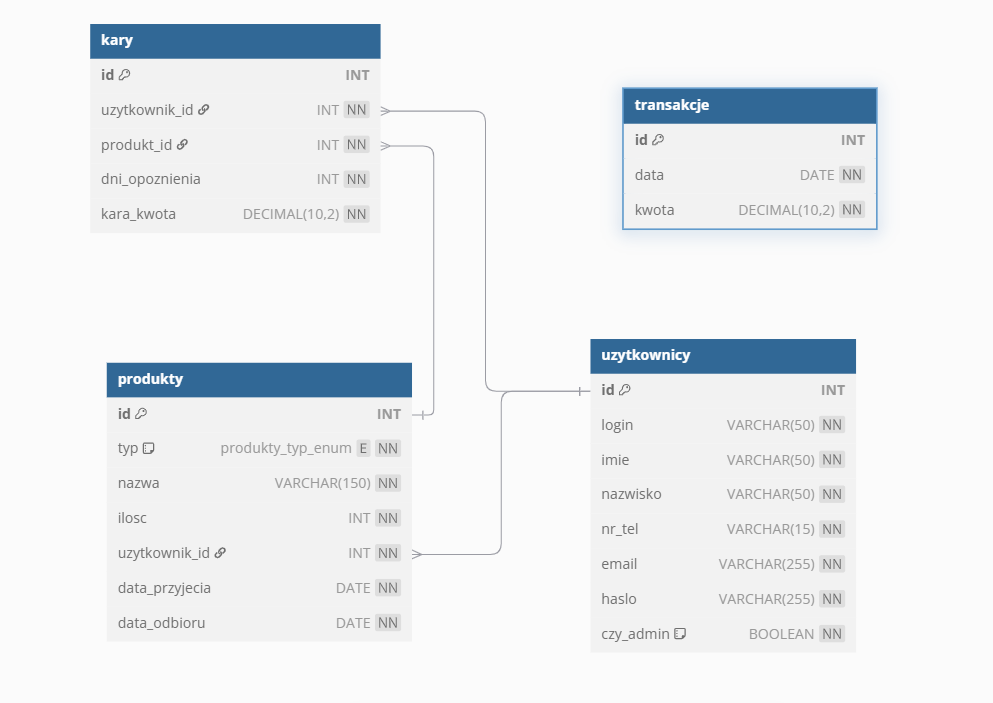
\includegraphics[width=.7\linewidth]{figures/SchematERD.png}\
    \caption{SchematERD.\label{schematERD}}
\end{figure}

\section{Kluczowe zależności oraz charakterystyka architektury}
\begin{itemize}
    \item \textbf{Dziedziczenie} - Wszystkie główne okna dziedziczą po \texttt{OknoBazowe}, co zapewnia spójny wygląd i zachowanie interfejsu użytkownika
    \item \textbf{Kompozycja} - Klasy serwisowe są używane przez panele użytkownika i administratora, a \texttt{DatabaseConnector} przez wszystkie klasy potrzebujące dostępu do bazy danych.
    \item \textbf{Modułowość} - Każda warstwa może być modyfikowana niezależnie od innych
    \item \textbf{Testowalność} - Logikę biznesową można testować w izolacji od warstwy prezentacji i danych
    \item \textbf{Spójność interfejsu} - Dzięki dziedziczeniu z \texttt{OknoBazowe} wszystkie okna mają jednolity wygląd
    \item \textbf{Bezpieczeństwo} - Walidacja danych na poziomie GUI i logiki biznesowej
\end{itemize}
\clearpage
\section{Wymagania systemowe}
Aby uruchomić projekt na własnym komputerze i móc go rozwijać, potrzebne jest kilka darmowych narzędzi. Poniższa lista wyjaśnia, co i dlaczego należy zainstalować.
\begin{itemize}
    \item \textbf{Pakiet XAMPP:} To gotowy zestaw narzędzi, który w prosty sposób instaluje serwer bazy danych. Jest on niezbędny, aby aplikacja miała gdzie przechowywać swoje dane.
    \item \textbf{Java Development Kit (JDK):} Jest to środowisko niezbędne do kompilowania i uruchamiania aplikacji napisanych w języku Java.
    \item \textbf{Środowisko IntelliJ IDEA:} To zaawansowany edytor kodu, w którym projekt był tworzony. Ułatwia on pracę z kodem, kompilację i uruchamianie programu.
\end{itemize}
Aktualne wymagania sprzętowe dla tych programów można znaleźć na ich oficjalnych stronach:
\begin{itemize}
    \item \textbf{XAMPP:} \url{https://www.apachefriends.org/download.html}
    \item \textbf{IntelliJ IDEA:} \url{https://www.jetbrains.com/help/idea/installation-guide.html#requirements}
\end{itemize}

\chapter{Harmonogram realizacji projektu}
\label{chap:Harmonogram realizacji projektu}

\begin{enumerate}
    \item \textbf{Dzień pierwszy}: Stworzenie podstawowej bazy danych oraz klasy \texttt{DatabaseConnector} oraz \texttt{Okno Bazowe}
    
    \item \textbf{Dzień drugi}: Ułożenie planu GUI, stworzenie takich klas jak \texttt{Walidacja}, \texttt{WygladPrzyciskow}, dodanie pakietu \texttt{Figures} oraz \texttt{logo.png}
    
    \item \textbf{Dzień trzeci}: Dodanie całego pakietu \texttt{serwis}
    
    \item \textbf{Dzień czwarty}: Dodanie \texttt{MenuGlowne} oraz zrobienie metody wywołania w \texttt{main}
    
    \item \textbf{Dzień piąty}: Dodanie \texttt{OknoLogowania}, \texttt{OknoRejestracji},  \texttt{PanelUzytkownika} oraz \texttt{PanelAdministratora}
    
    \item \textbf{Dzień szósty}: Ostatnie poprawki i testy oraz dokumentacja
\end{enumerate}

\begin{figure}[H]
    \centering
    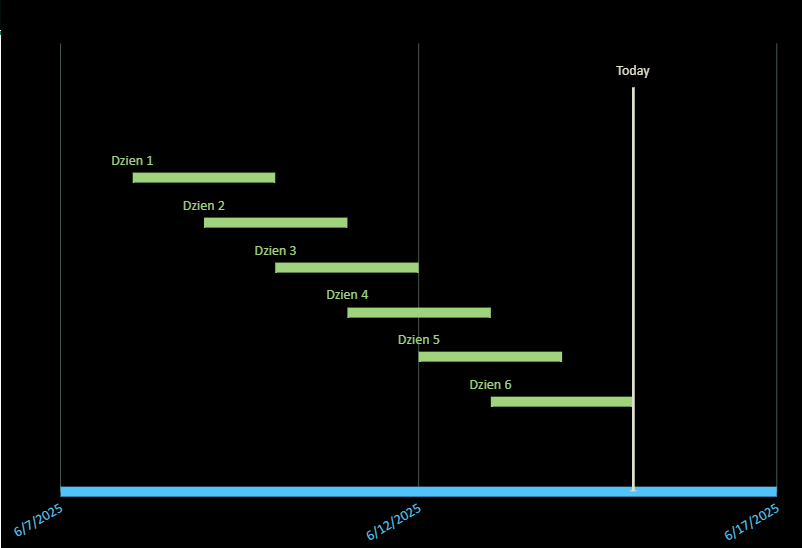
\includegraphics[width=.9\linewidth]{figures/SchematGrantta.png}\
    \caption{SchematGrantta.\label{SchematGrantta}}
\end{figure}


\chapter{Prezentacja warstwy użytkowej projektu}
\label{chap:Prezentacja warstwy użytkowej projektu}
Cały projekt znajduje się na moim repozytorium: \url{https://github.com/MarcinKida/ProjektJava/tree/master}
Baza danych do tego projektu jest zamieszczona w README.md 
Użytkownik utworzony w bazie danych ma login admin, natomiast jego hasło to admin1
\section{MenuGlowne}
\label{sec:MenuGlowne}
Pierwsze rzeczą jaka ukaże się użytkownikowi po uruchomieniu programu jest MenuGlowne. Jest ono przedstawione na rysunku poniżej.
\begin{figure}[H]
    \centering
    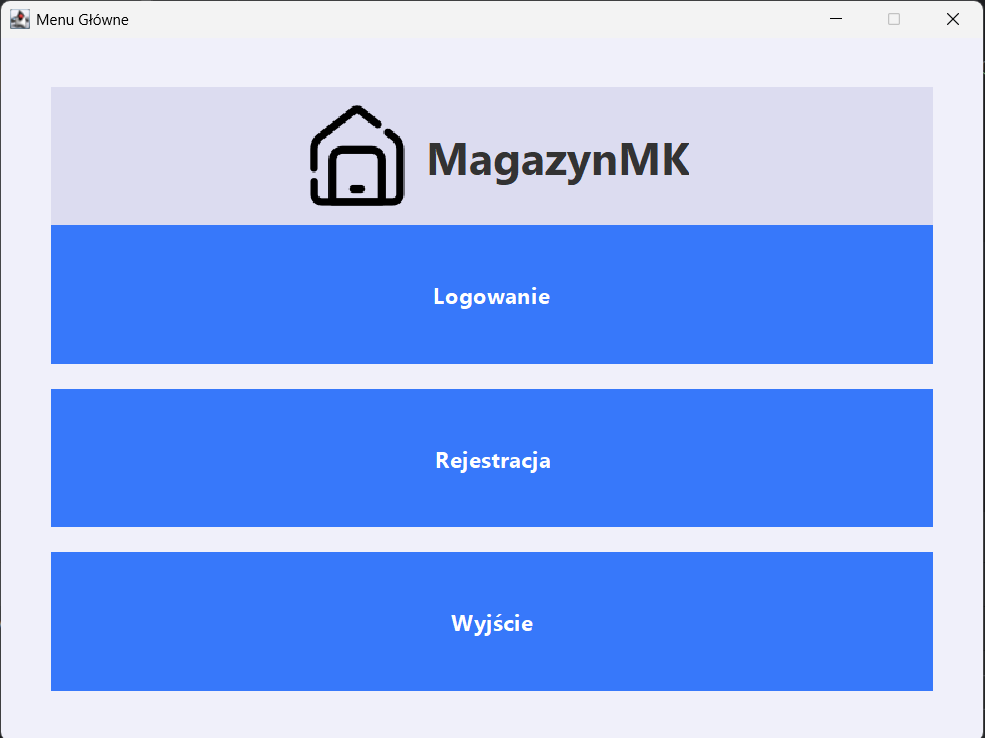
\includegraphics[width=.7\linewidth]{figures/MenuGlowne.png}\
    \caption{MenuGlowne.\label{MenuGlowne}}
\end{figure}
\clearpage
Po kliknięciu przycisku Wyjscie GUI się wyłącza. Natomiast po kliknięciu Zarejestruj przenosi nas do OknoRejestracji
\section{OknoRejestracji}
\label{sec:OknoRejestracji}

Tak wygląda okno rejestracji
\begin{figure}[H]
    \centering
    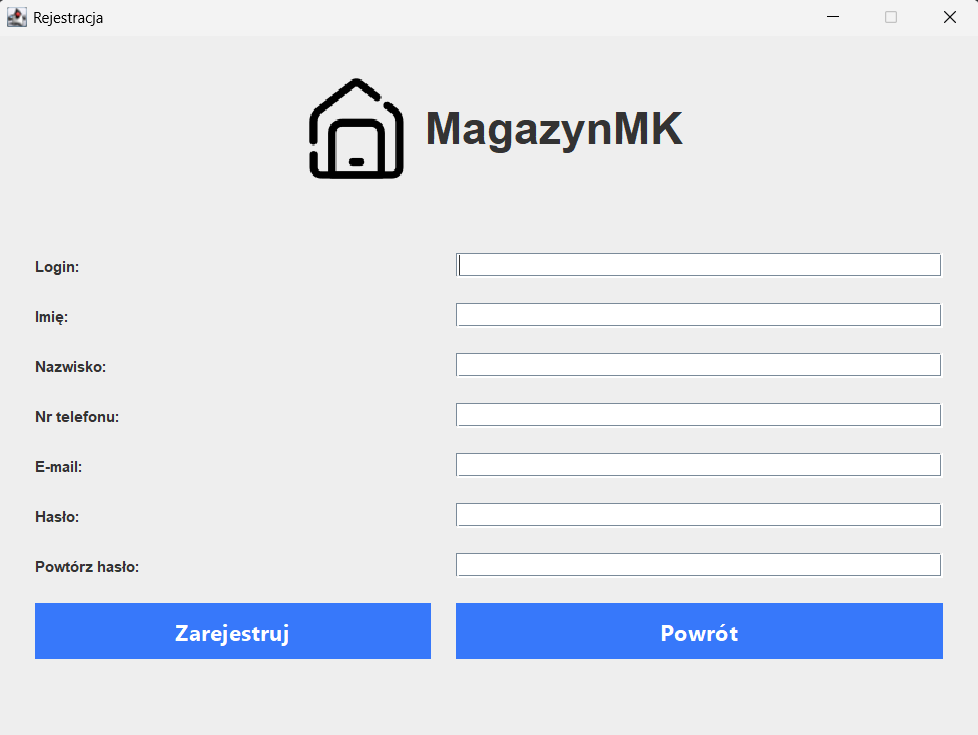
\includegraphics[width=.7\linewidth]{figures/OknoRejestracji.png}\
    \caption{OknoRejestracji.\label{OknoRejestracji}}
\end{figure}
Jeśli login ma mniej niż 4 litery lub cyfry wyskakuje taki komunikat:
\begin{figure}[H]
    \centering
    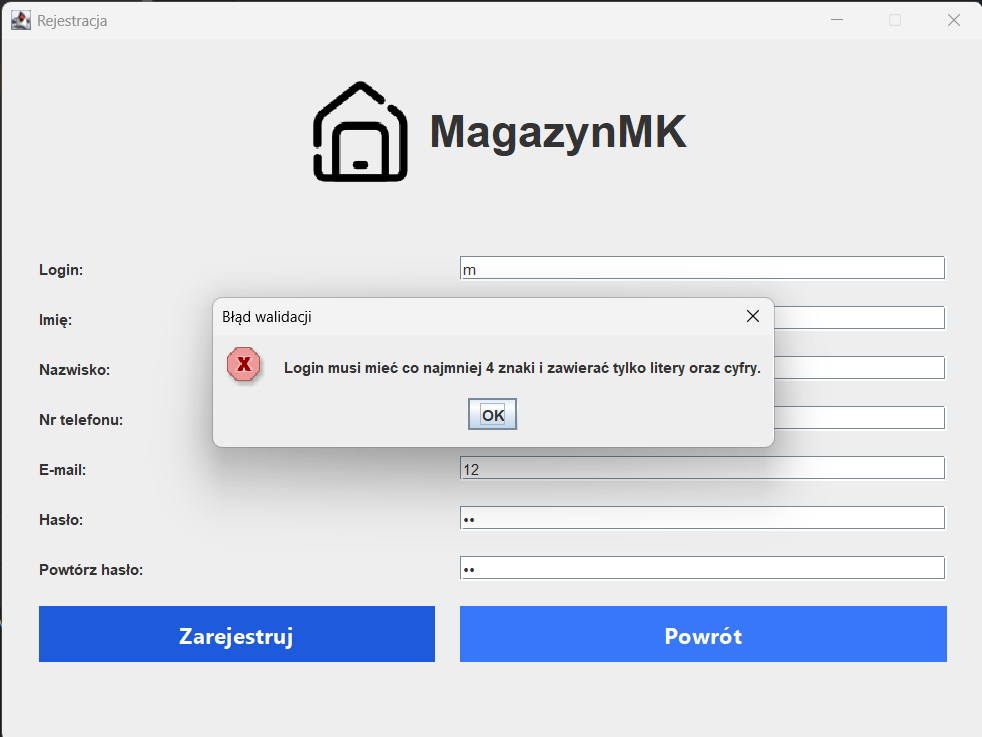
\includegraphics[width=.7\linewidth]{figures/RejestracjaKom1.png}\
    \caption{Komunikat1.\label{Komunikat1}}
\end{figure}
Jeśli Nr.Tel nie ma od 9 do 11 cyfr wyrzuca taki komunikat:
\begin{figure}[H]
    \centering
    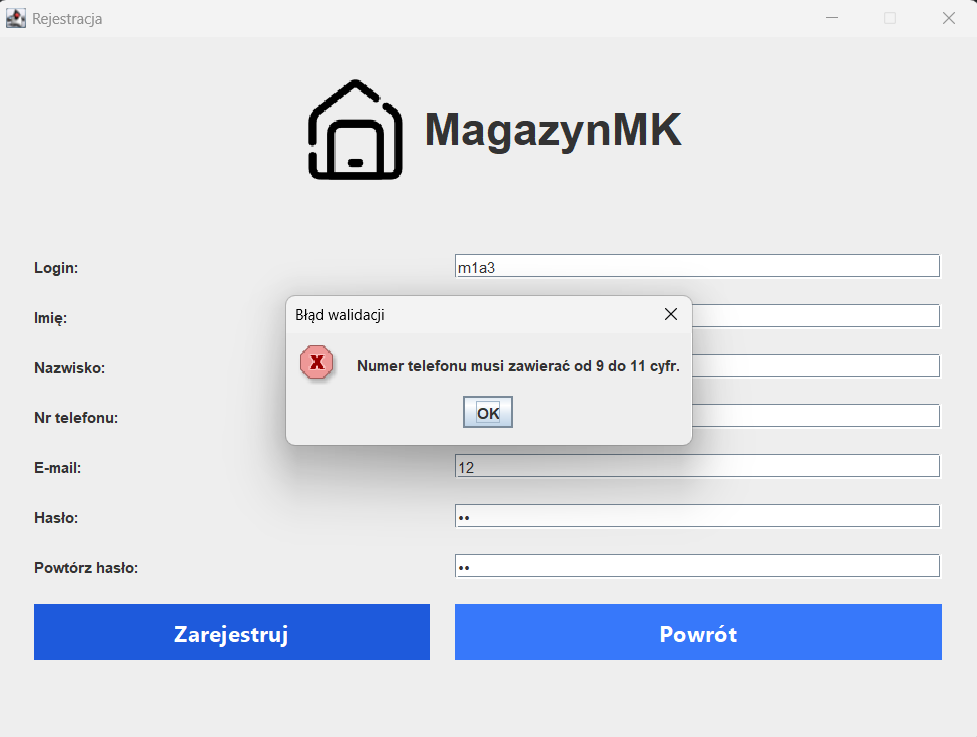
\includegraphics[width=.7\linewidth]{figures/RejestracjaKom2.png}\
    \caption{Komunikat2.\label{Komunikat2}}
\end{figure}
Jeśli email nie ma w sobie "@" wyrzuca taki komunikat:
\begin{figure}[H]
    \centering
    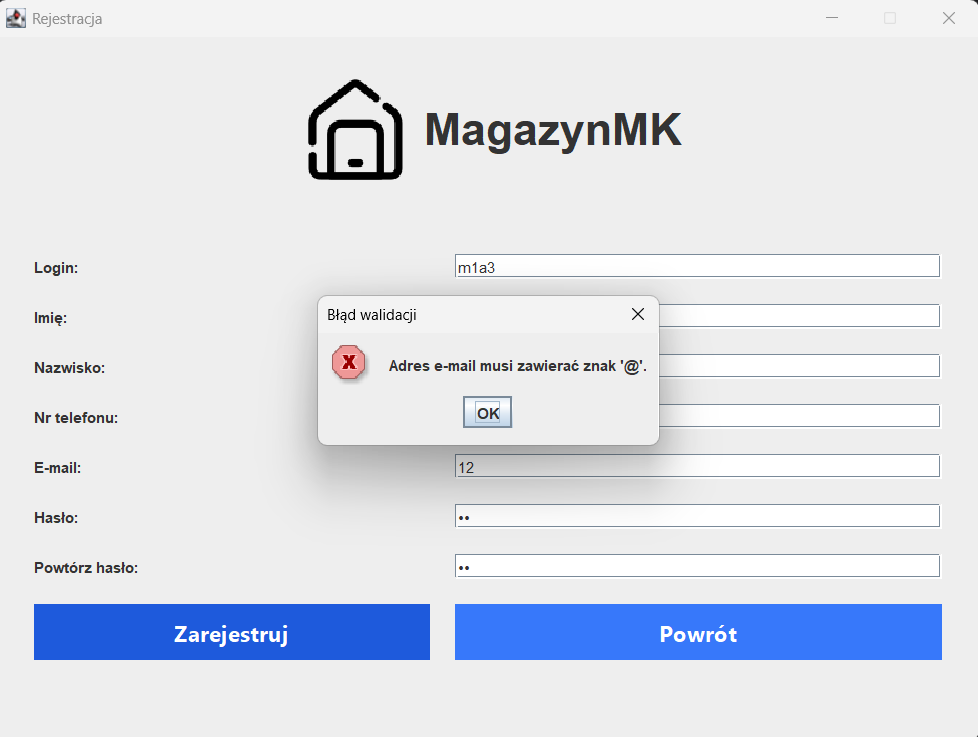
\includegraphics[width=.7\linewidth]{figures/RejestracjaKom3.png}\
    \caption{Komunikat3.\label{Komunikat3}}
\end{figure}
Jeśli hasła się nie pokrywają wyświetla taki komunikat:
\begin{figure}[H]
    \centering
    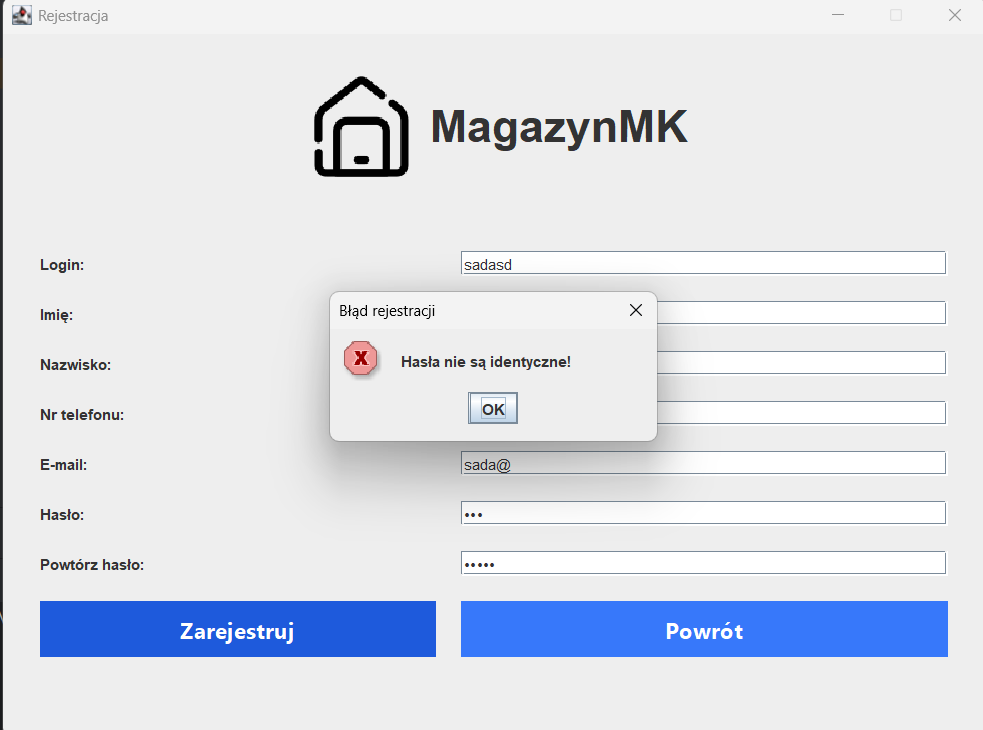
\includegraphics[width=.7\linewidth]{figures/RejestracjaKom4.png}\
    \caption{Komunikat4.\label{Komunikat4}}
\end{figure}
Jeśli dane zostały wpisane poprawne wypisuje taki komunikat:
\begin{figure}[H]
    \centering
    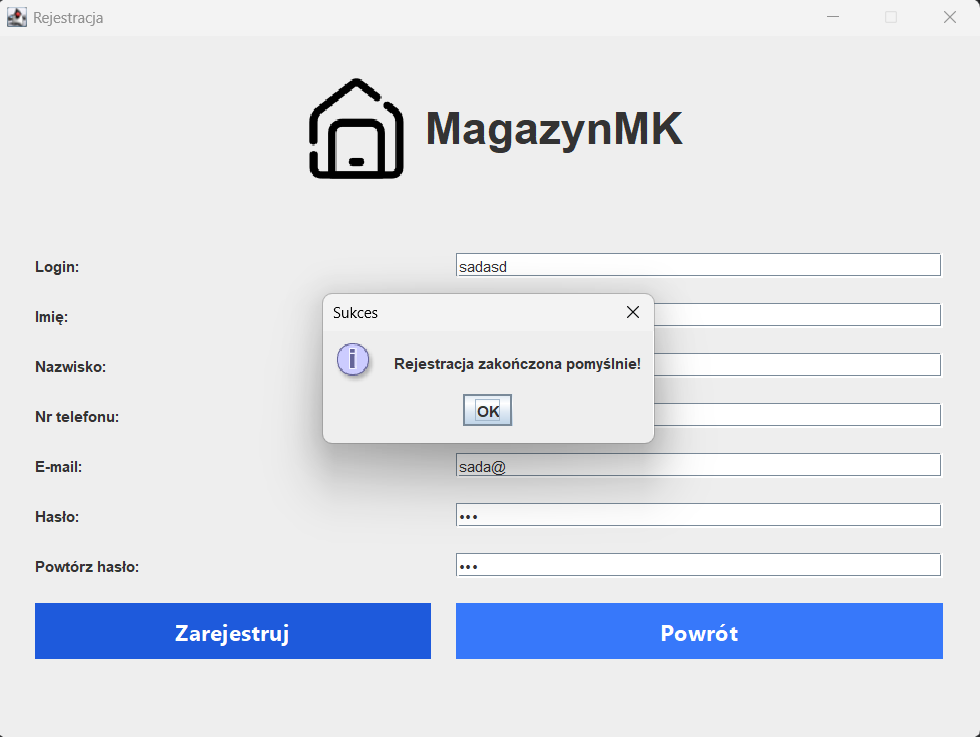
\includegraphics[width=.7\linewidth]{figures/RejestracjaKom5.png}\
    \caption{Komunikat5.\label{Komunikat5}}
\end{figure}
Po kliknięciu ok przechodzi do OknoLogowania
\clearpage
\section{OknoLogowania}
\label{sec:OknoLogowania}
Po kliknięciu w MenuGlowne przycisku Zaloguj lub po zarejestrowaniu się wyskakuje nam okno logowania:
\begin{figure}[H]
    \centering
    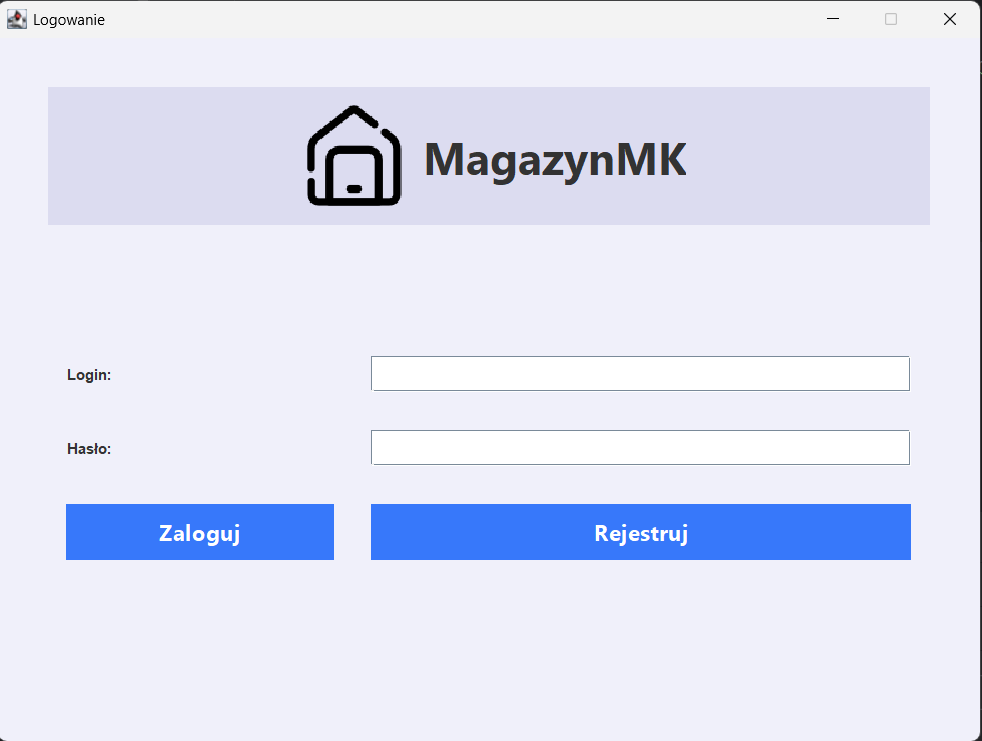
\includegraphics[width=.7\linewidth]{figures/OknoLogowania.png}\
    \caption{OknoLogowania.\label{OknoLogowania}}
\end{figure}
Jeśli wpiszemy niepoprawne dane wyskoczy komunikat:
\begin{figure}[H]
    \centering
    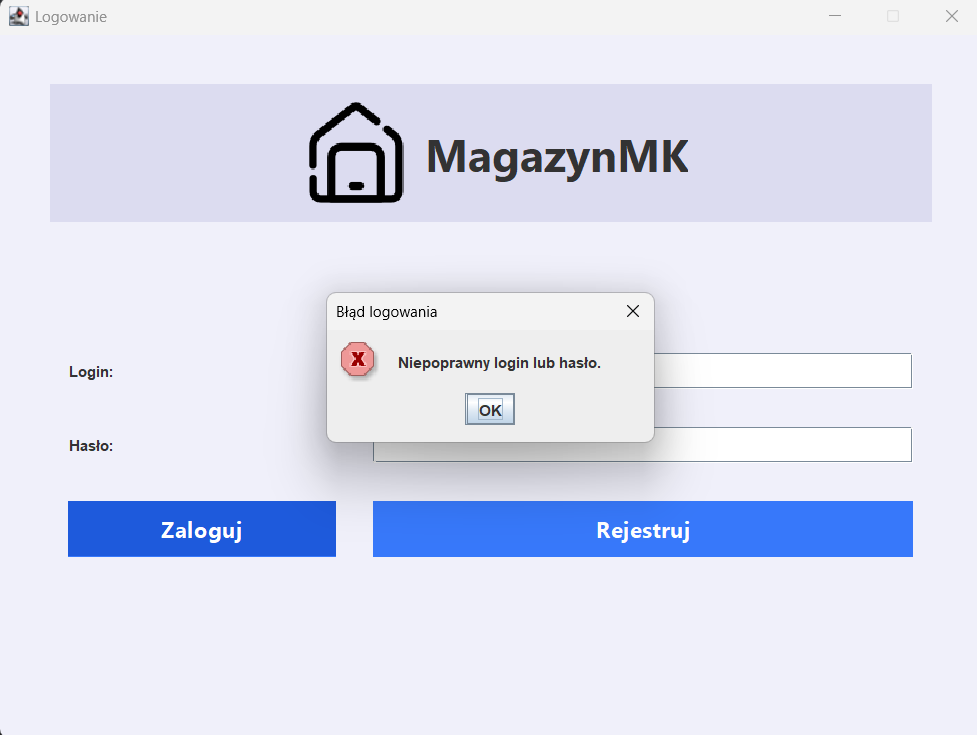
\includegraphics[width=.7\linewidth]{figures/LogowanieKomunikat.png}\
    \caption{Komunikat6.\label{Komunikat6}}
\end{figure}
\clearpage
\section{PanelUzytkownika}
\label{sec:PanelUzytkownika}
Jeśli w oknie logowania zalogujemy się na konto użytkownika nie będącego administratorem wyskoczy nam PanelUzytkownika:
\begin{figure}[H]
    \centering
    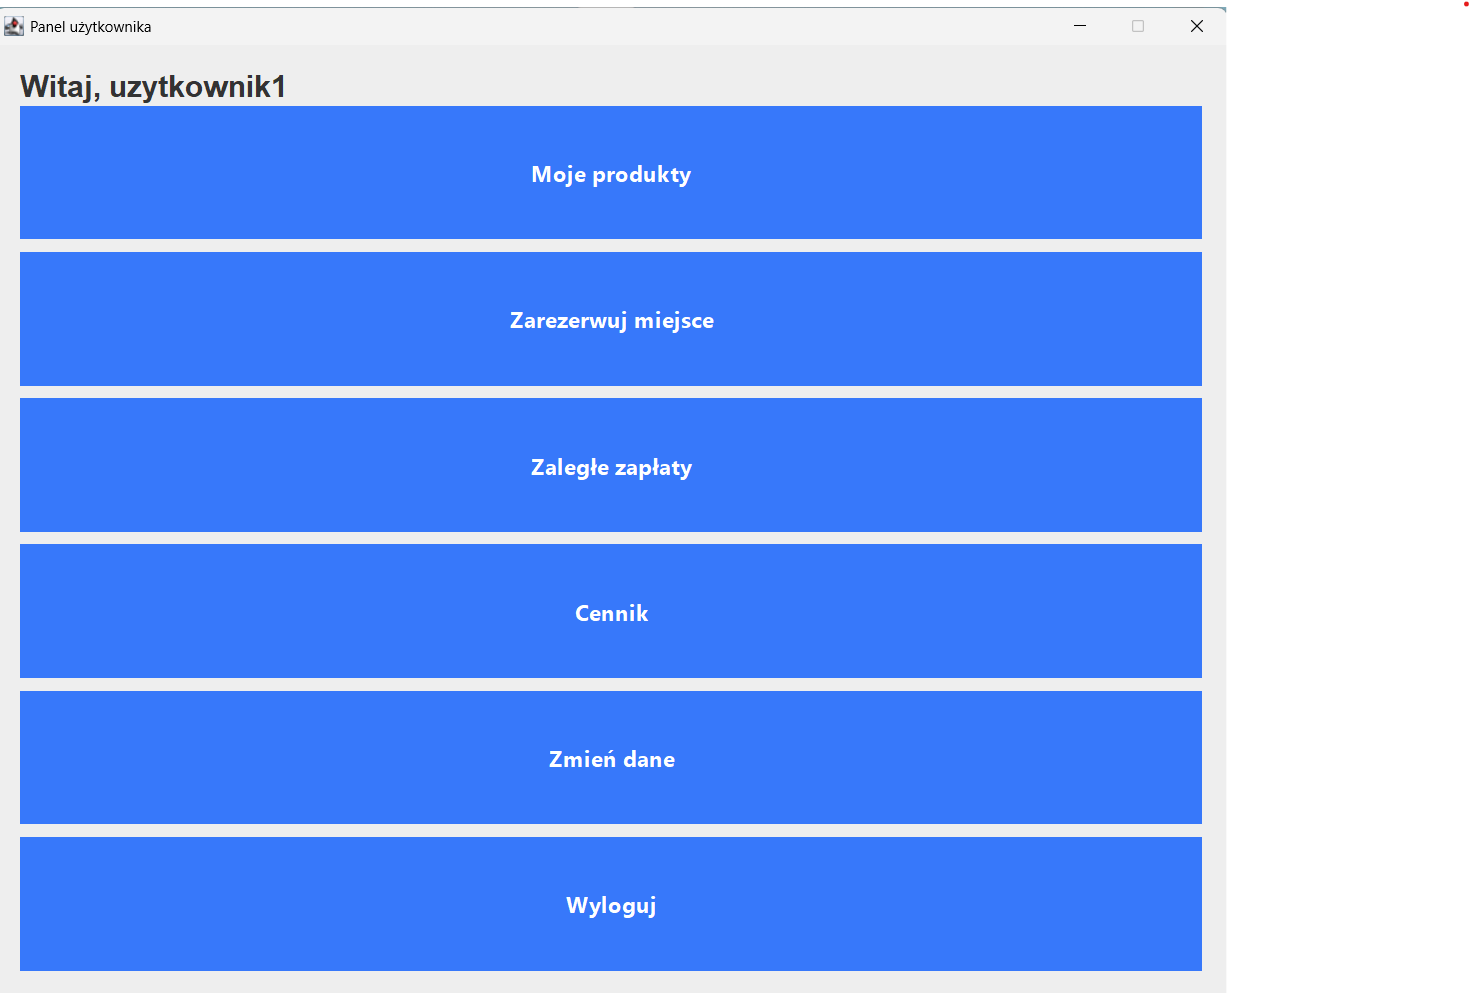
\includegraphics[width=.7\linewidth]{figures/PanelUzytkownika.png}\
    \caption{PanelUzytkownika.\label{PanelUzytkownika}}
\end{figure}
\clearpage
\subsection{Moje produkty}
\label{subsec:Moje produkty}
Po kliknięciu Moje Produkty wyskoczy nam takie okienko:
\begin{figure}[H]
    \centering
    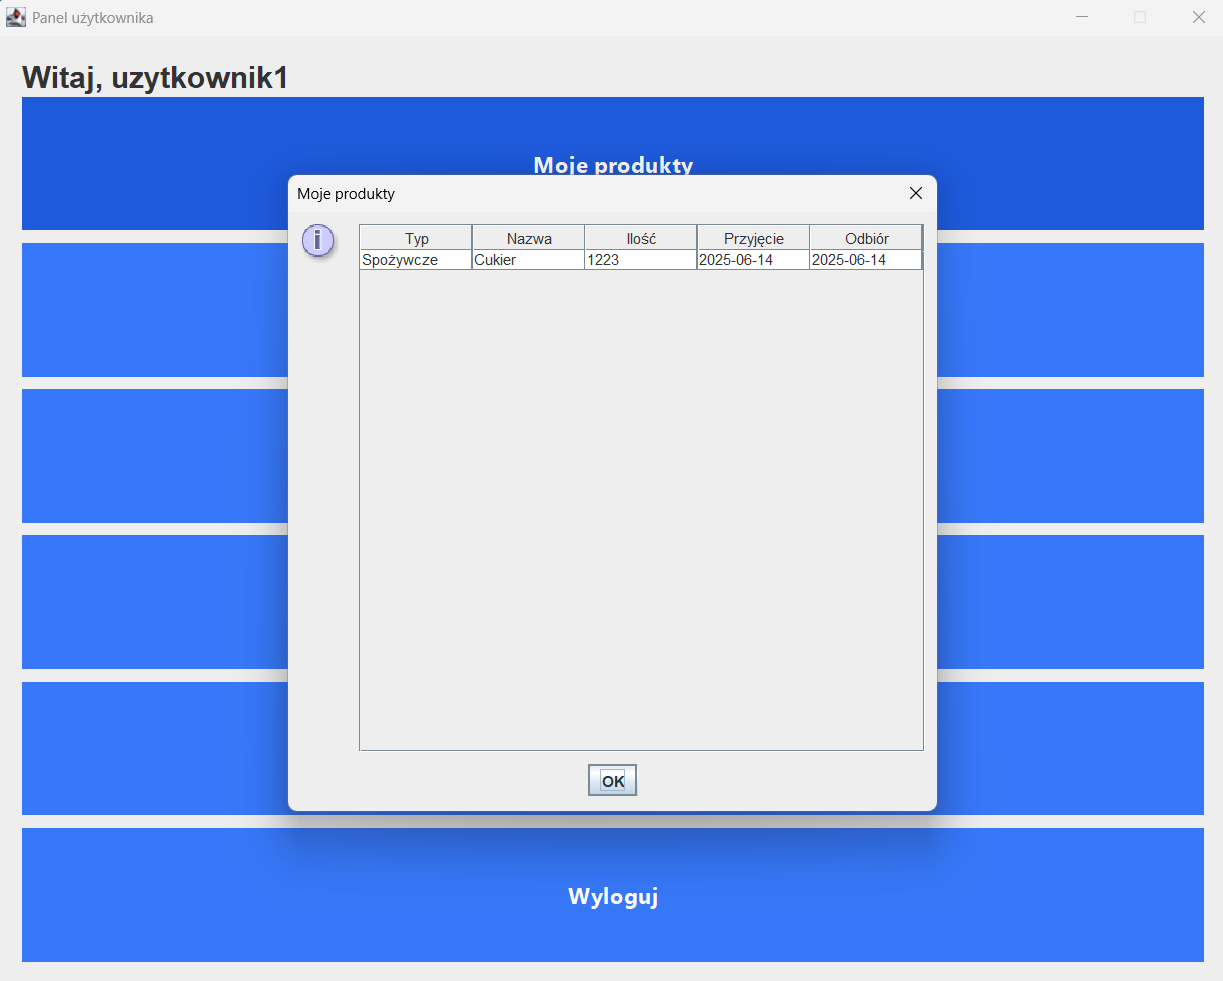
\includegraphics[width=.7\linewidth]{figures/PanelUzytkownika1.png}\
    \caption{PanelUzytkownika1.\label{PanelUzytkownika1}}
\end{figure}
\clearpage
\subsection{Zarezerwuj miejsce}
\label{subsec:Zarezerwuj miejsce}
Po kliknięciu na Zarezerwuj miejsce wyskakuje takie okno:
\begin{figure}[H]
    \centering
    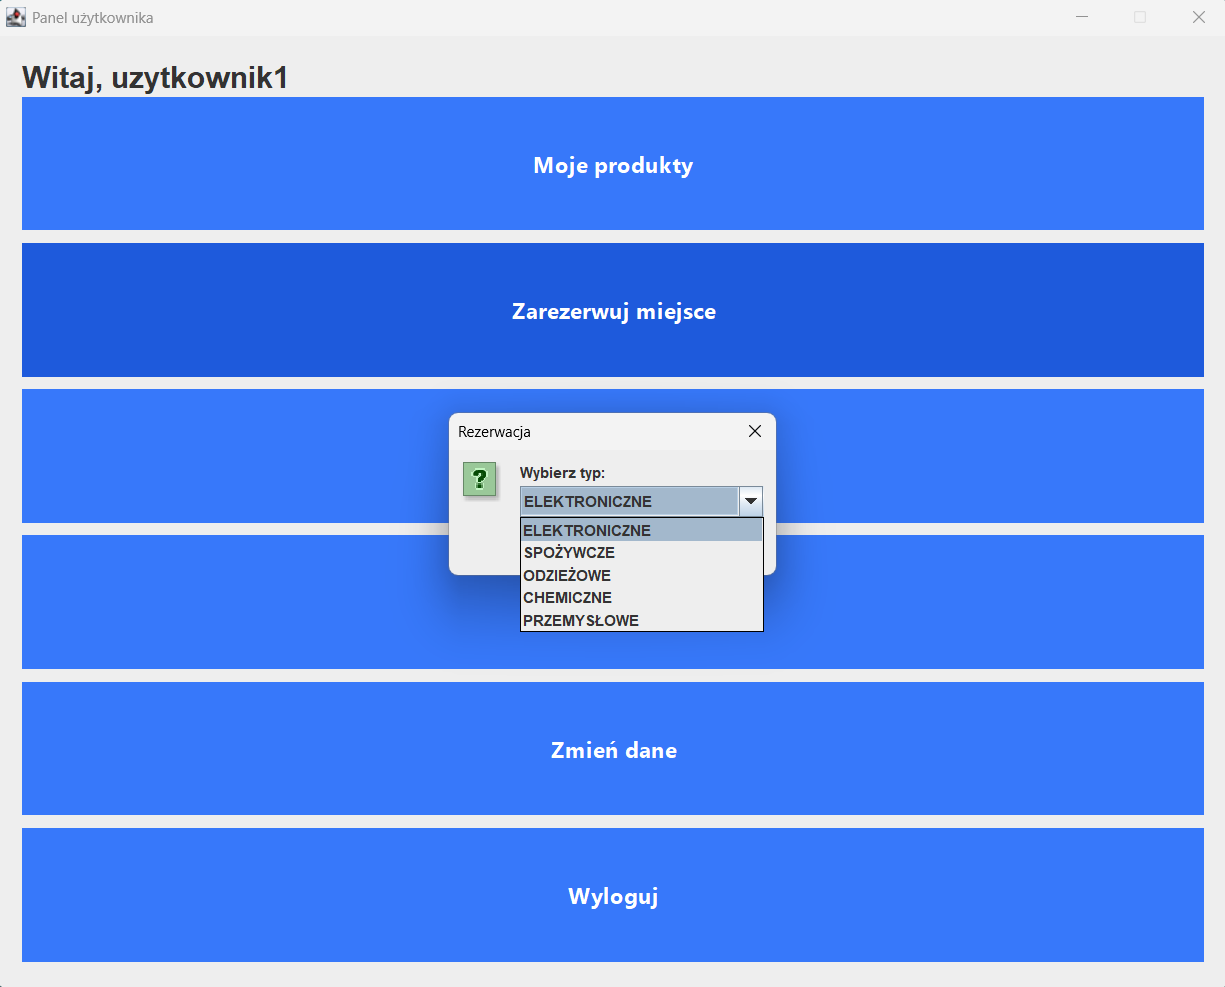
\includegraphics[width=.7\linewidth]{figures/PanelUzytkownika2.png}\
    \caption{PanelUzytkownika2.\label{PanelUzytkownika2}}
\end{figure}
Do każdego typu produktu są przypisane po 3 rodzaje produktów:
ELEKTRONICZNE:
\begin{figure}[H]
    \centering
    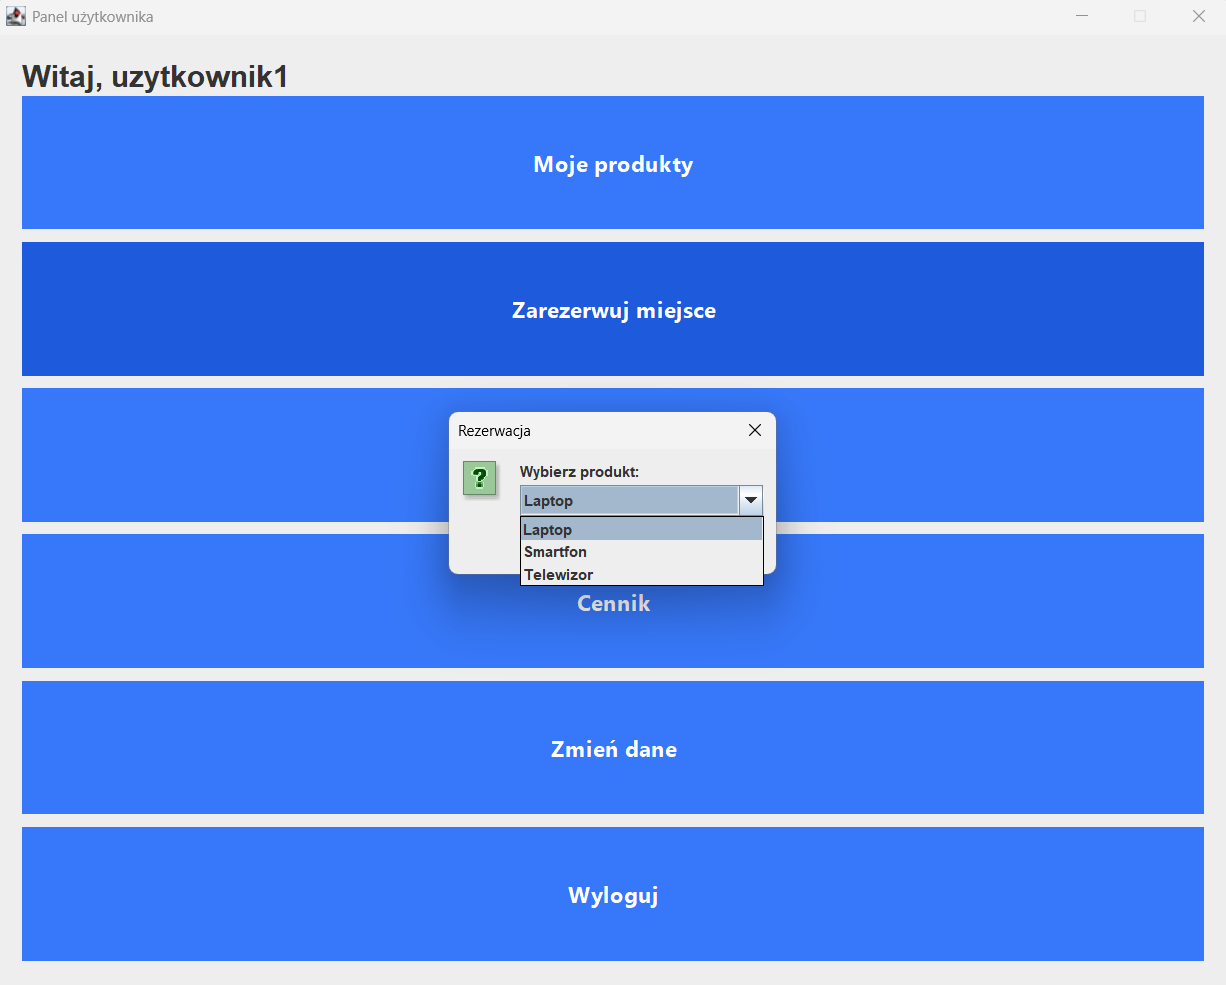
\includegraphics[width=.7\linewidth]{figures/PanelUzytkownika3.png}\
    \caption{PanelUzytkownika3.\label{PanelUzytkownika3}}
\end{figure}
SPOŻYWCZE:
\begin{figure}[H]
    \centering
    \includegraphics[width=.7\linewidth]{figures/PanelUzytkownika9.png}\
    \caption{PanelUzytkownika9.\label{PanelUzytkownika9}}
\end{figure}
ODZIEŻOWE:
\begin{figure}[H]
    \centering
    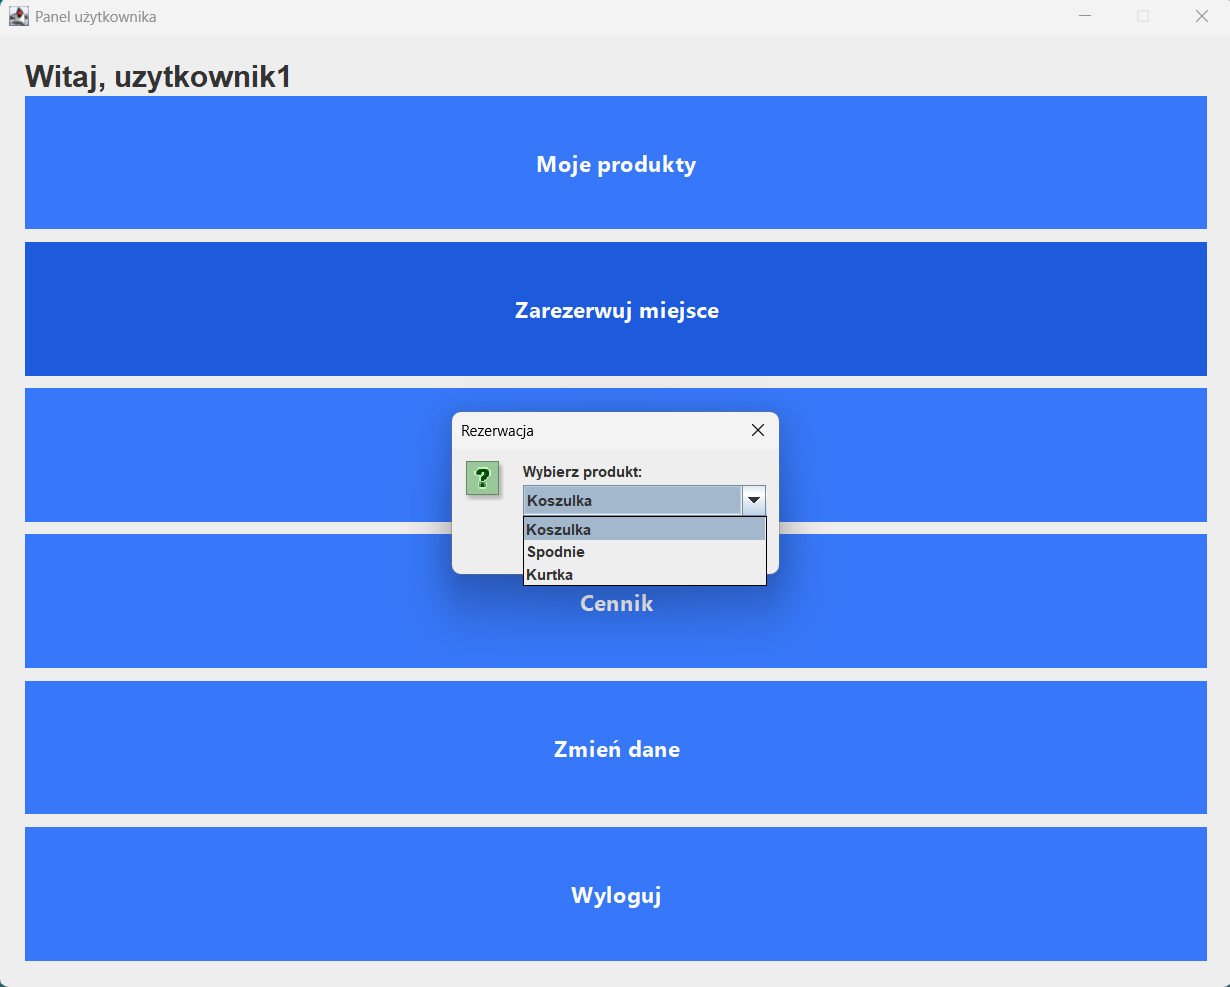
\includegraphics[width=.7\linewidth]{figures/PanelUzytkownika10.png}\
    \caption{PanelUzytkownika10.\label{PanelUzytkownika10}}
\end{figure}
CHEMICZNE:
\begin{figure}[H]
    \centering
    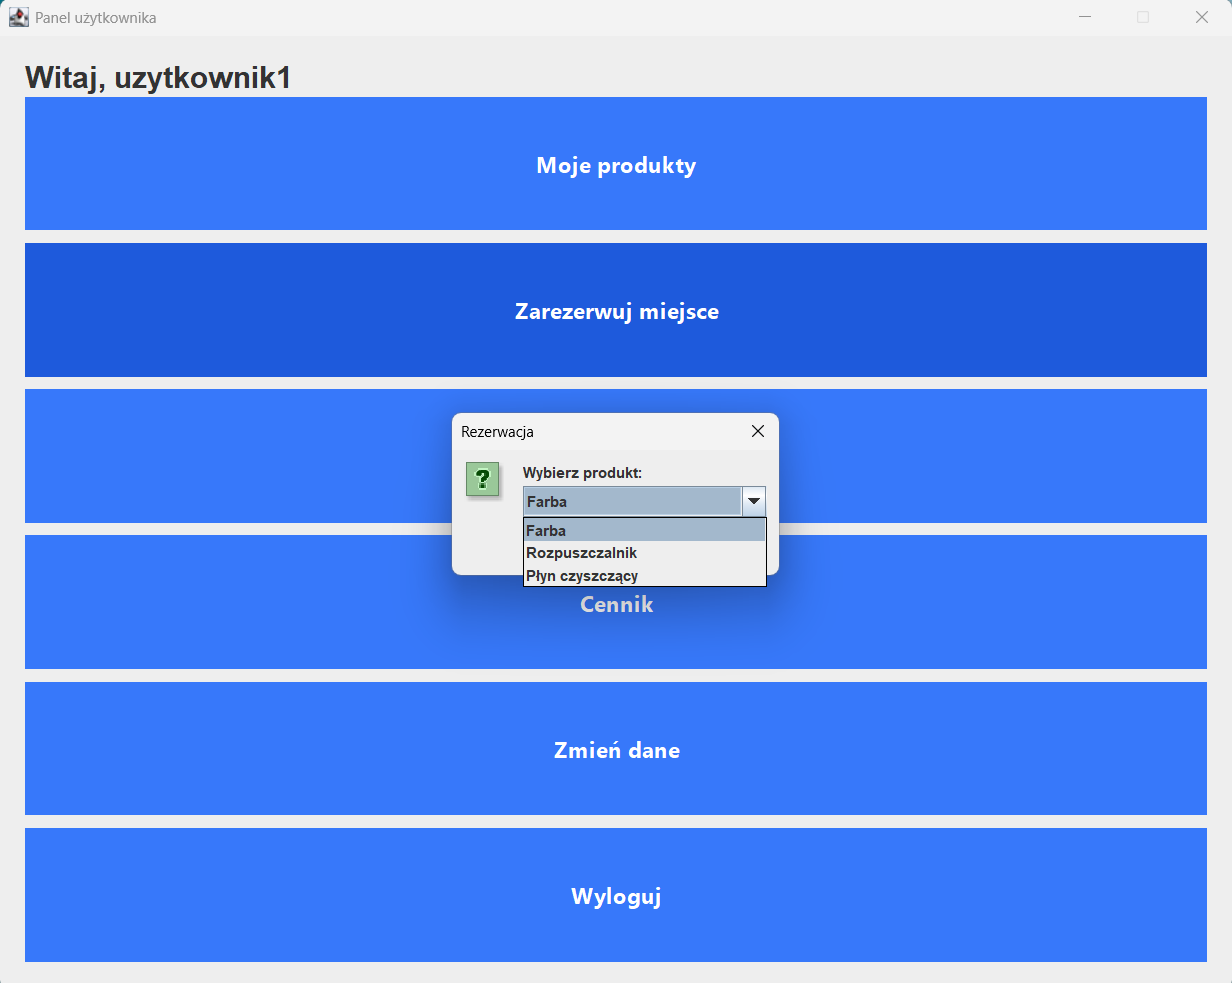
\includegraphics[width=.7\linewidth]{figures/PanelUzytkownika11.png}\
    \caption{PanelUzytkownika11.\label{PanelUzytkownika11}}
\end{figure}
PRZEMYSŁOWE:
\begin{figure}[H]
    \centering
    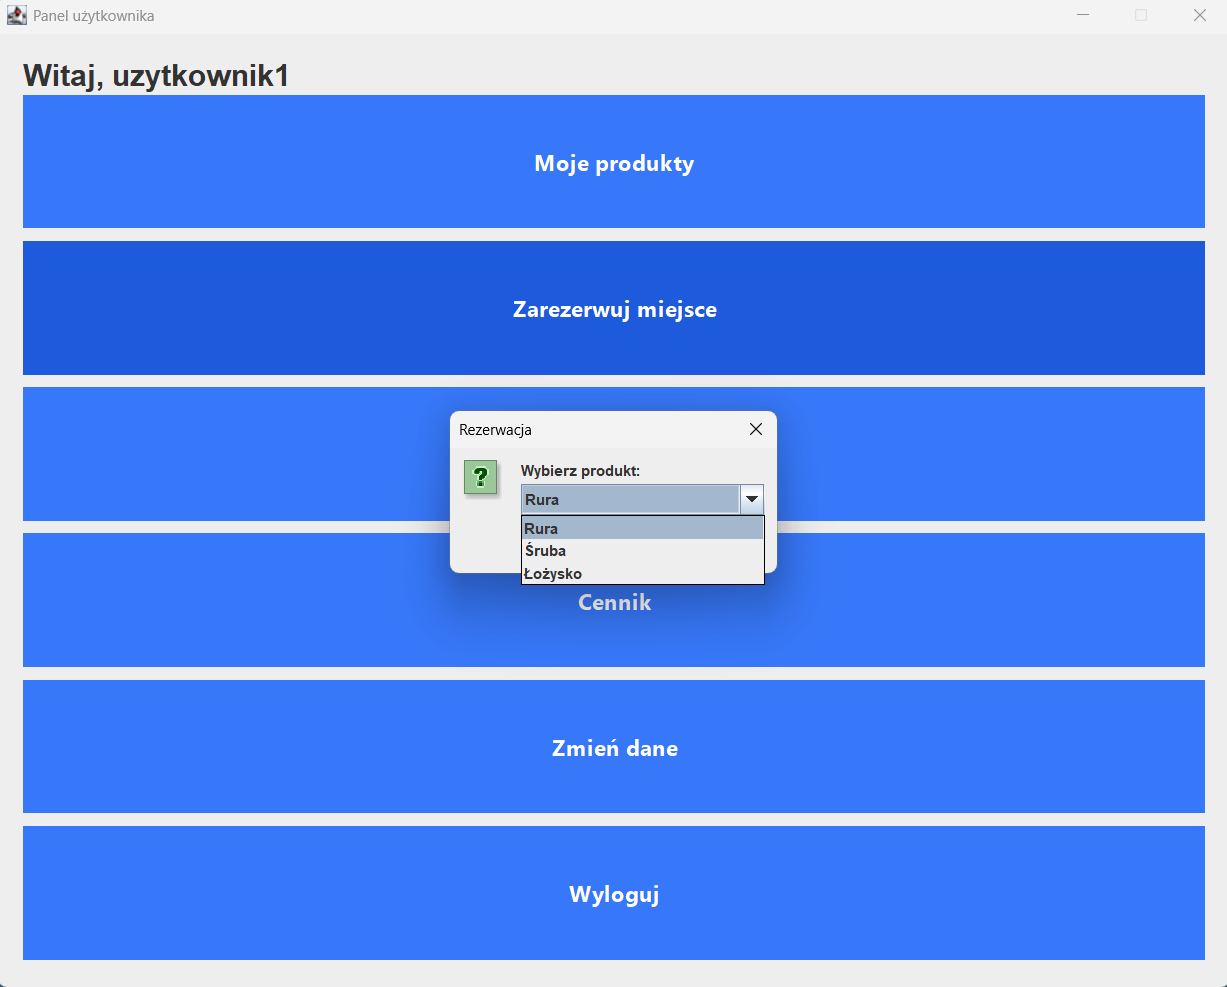
\includegraphics[width=.7\linewidth]{figures/PanelUzytkownika12.png}\
    \caption{PanelUzytkownika12.\label{PanelUzytkownika12}}
\end{figure}
Po wybraniu produktu musimy wpisać ilość:
\begin{figure}[H]
    \centering
    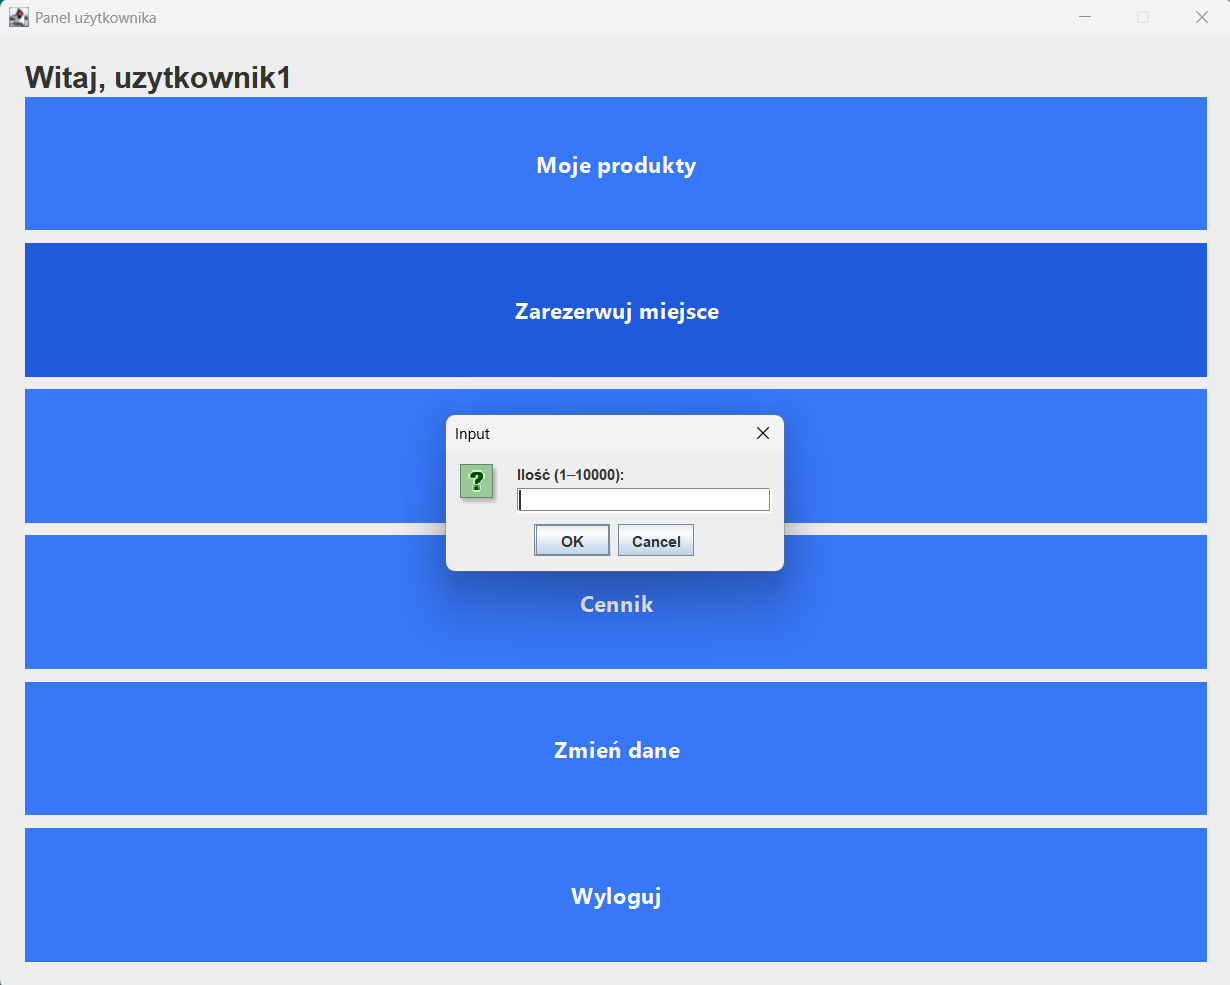
\includegraphics[width=.7\linewidth]{figures/Paneluzytkownika4.png}\
    \caption{PanelUzytkownika4.\label{PanelUzytkownika4}}
\end{figure}
Jeśli ilość przekroczy 10000, to wyskoczy taki komunikat:
\begin{figure}[H]
    \centering
    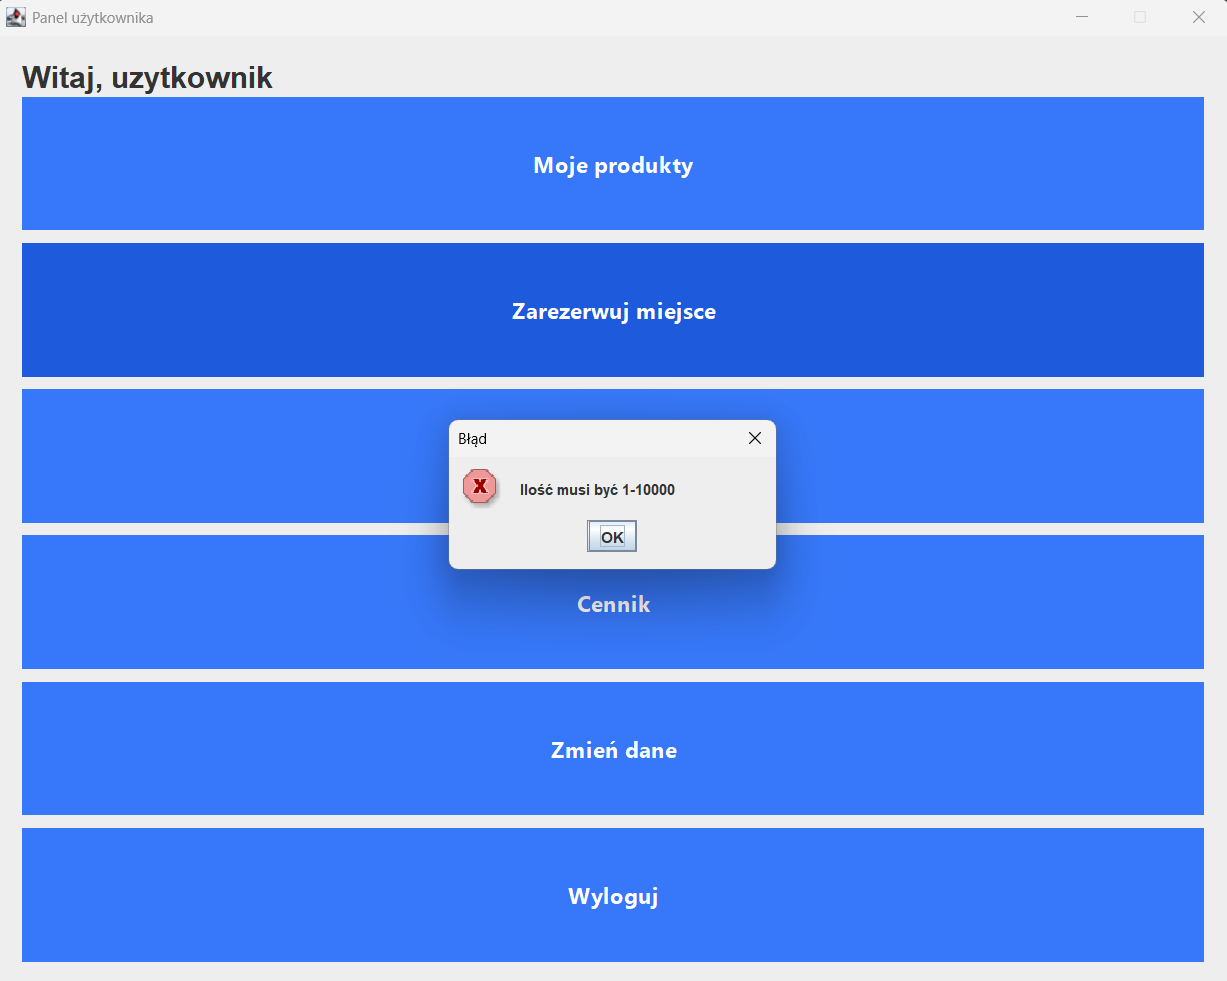
\includegraphics[width=.7\linewidth]{figures/PanelUzytkownika23.png}\
    \caption{PanelUzytkownika23.\label{PanelUzytkownika23}}
\end{figure}
Następnie należy wybrać daty od kiedy do kiedy rezerwujemy miejsce:
\begin{figure}[H]
    \centering
    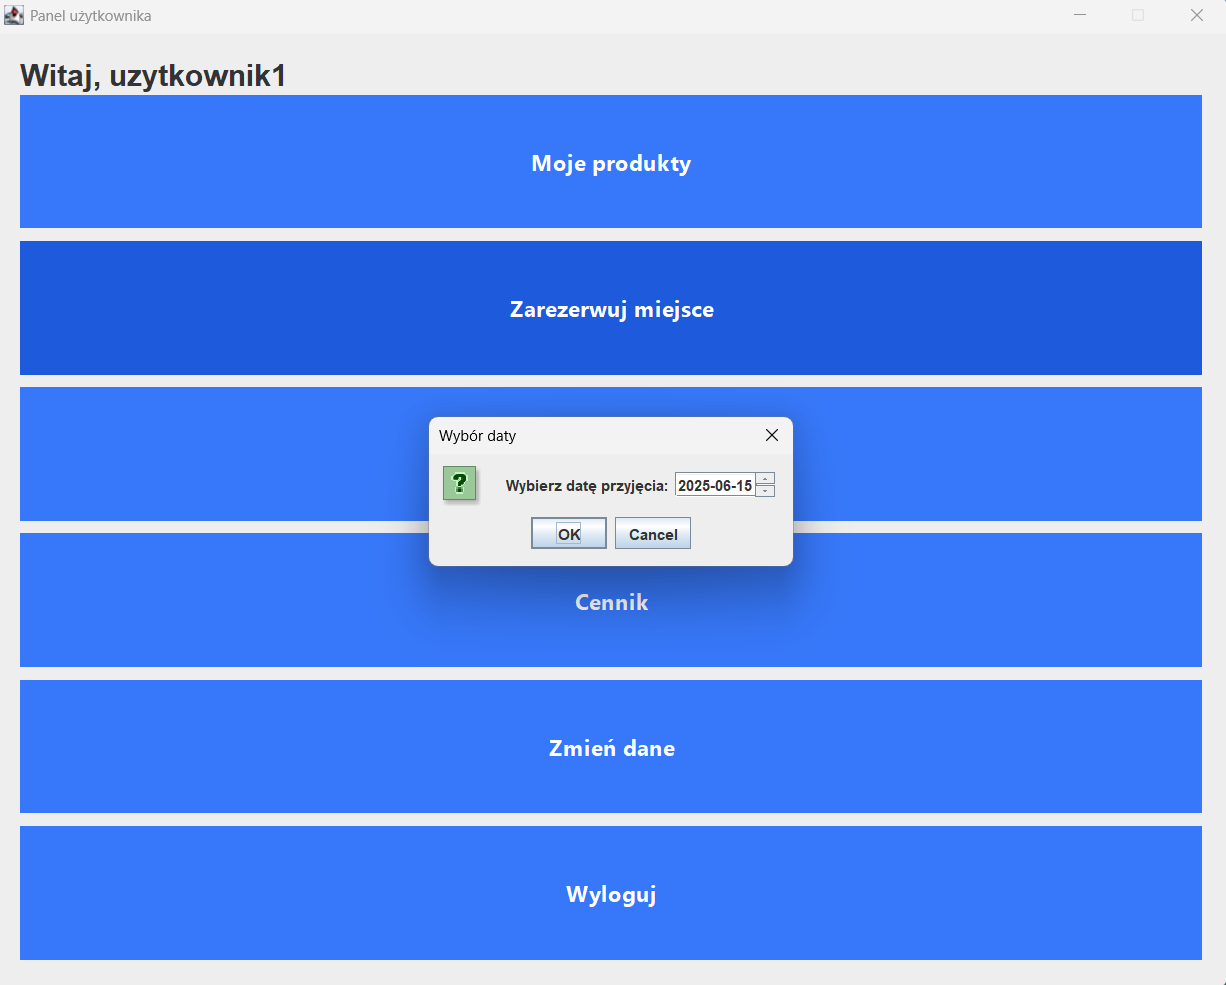
\includegraphics[width=.7\linewidth]{figures/PanelUzytkownika5.png}\
    \caption{PanelUzytkownika5.\label{PanelUzytkownika5}}
\end{figure}
\begin{figure}[H]
    \centering
    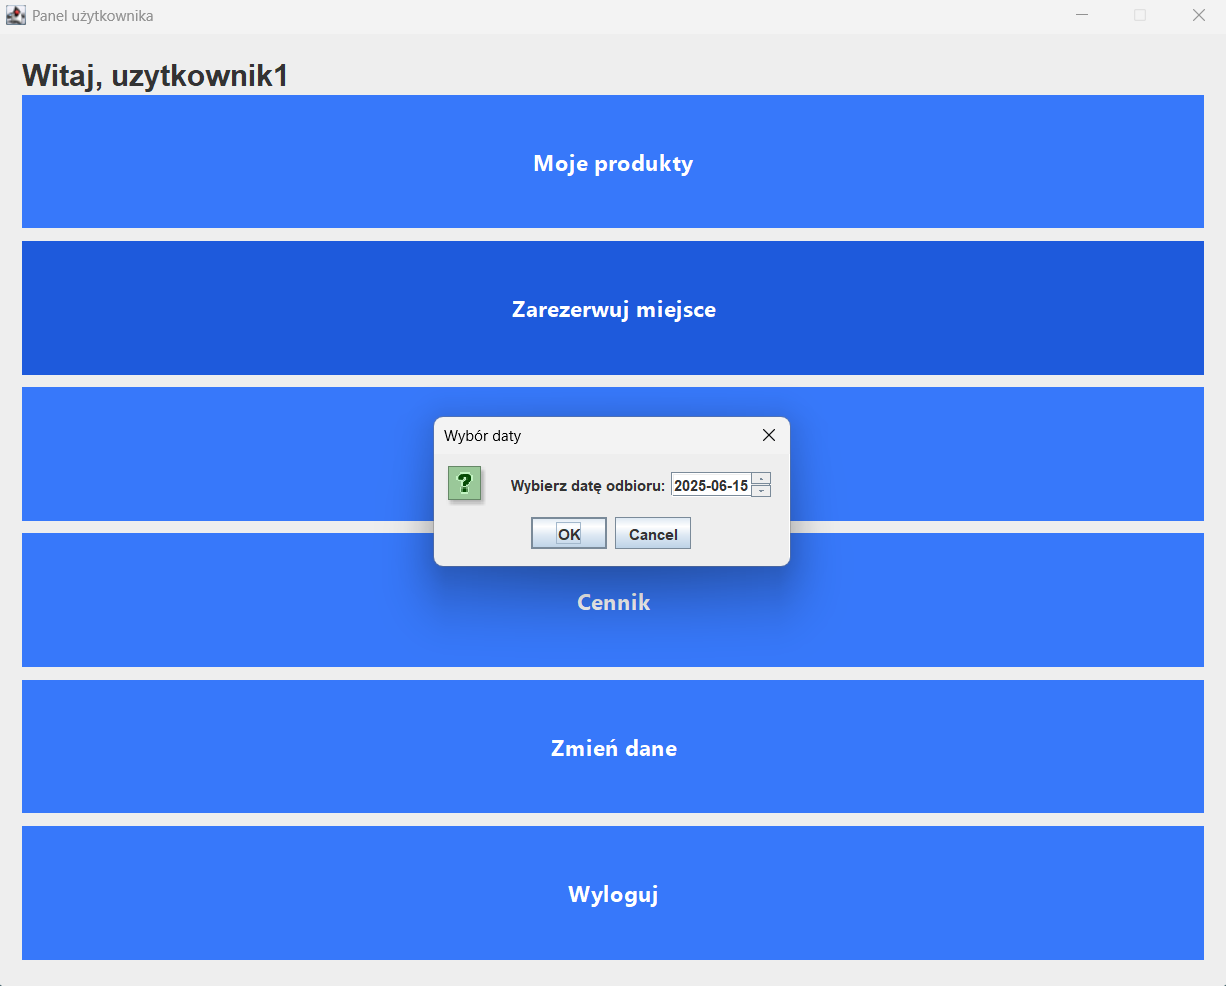
\includegraphics[width=.7\linewidth]{figures/PanelUzytkownika6.png}\
    \caption{PanelUzytkownika6.\label{PanelUzytkownika6}}
\end{figure}
Następnie wyświetla 2 komunikaty:
\begin{figure}[H]
    \centering
    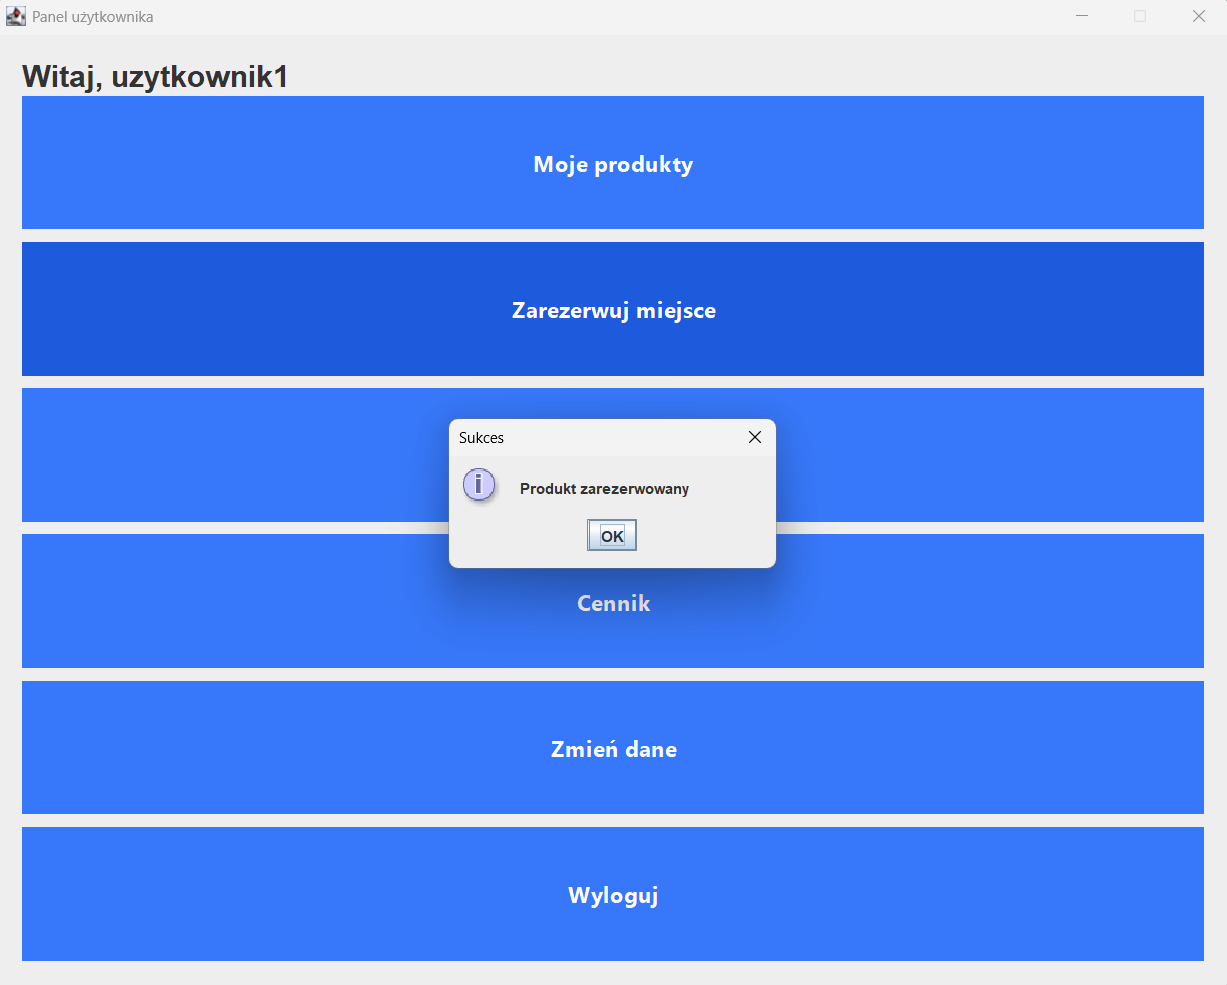
\includegraphics[width=.7\linewidth]{figures/PanelUzytkownika7.png}\
    \caption{PanelUzytkownika7.\label{PanelUzytkownika7}}
\end{figure}
Drugi komunikat mówi nam o kwocie(oblicza ją według cennika) oraz informuje o adresie na którym trzeba uiścić opłatę:
\begin{figure}[H]
    \centering
    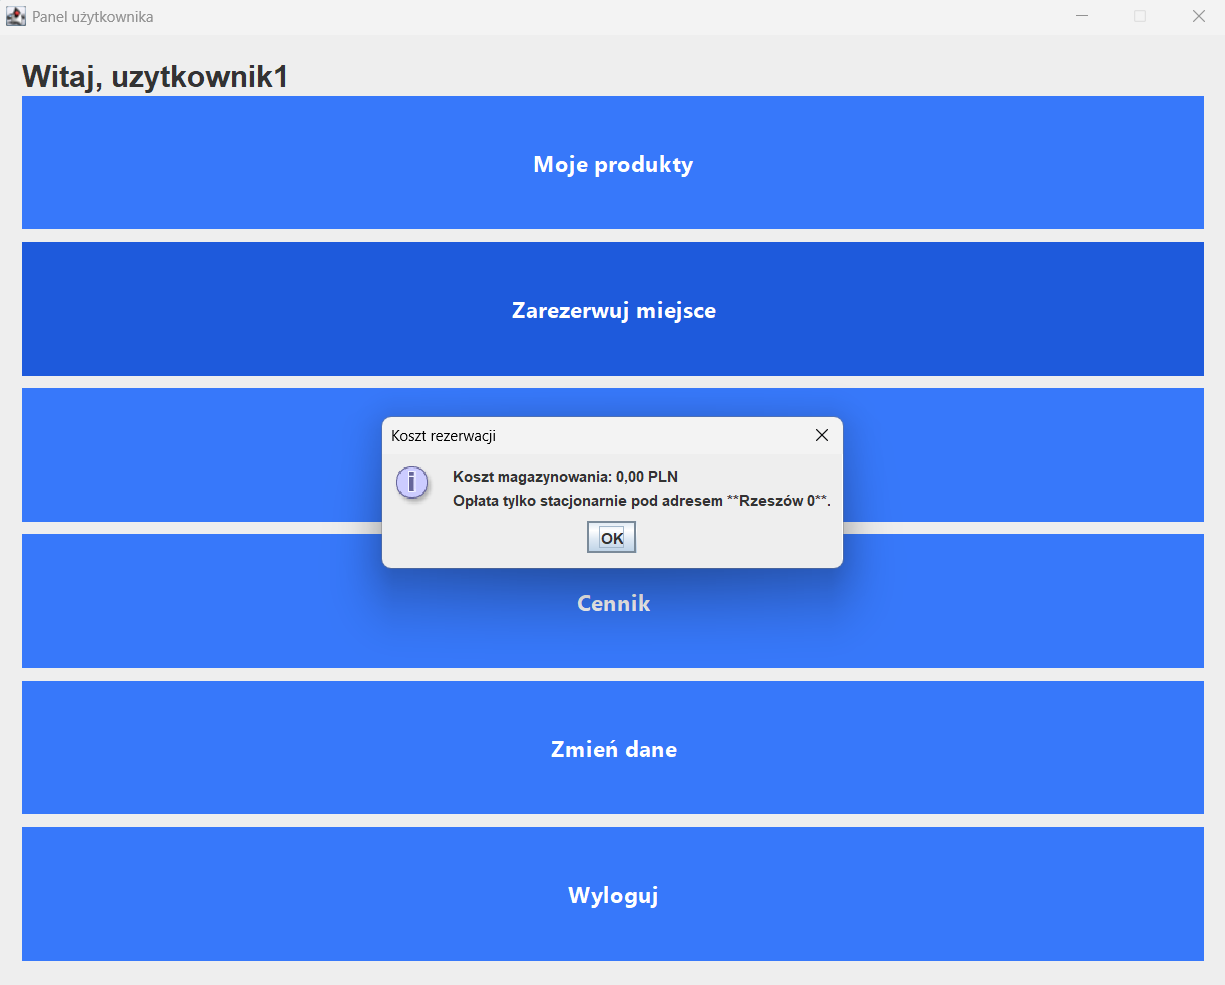
\includegraphics[width=.7\linewidth]{figures/PanelUzytkownika8.png}\
    \caption{PanelUzytkownika8.\label{PanelUzytkownika8}}
\end{figure}
\clearpage
\subsection{Zaległe kary}
\label{subsec:Zaległe kary}
Po kliknięciu na Zaległe zapłaty wyświetli nam się tabela:
\begin{figure}[H]
    \centering
    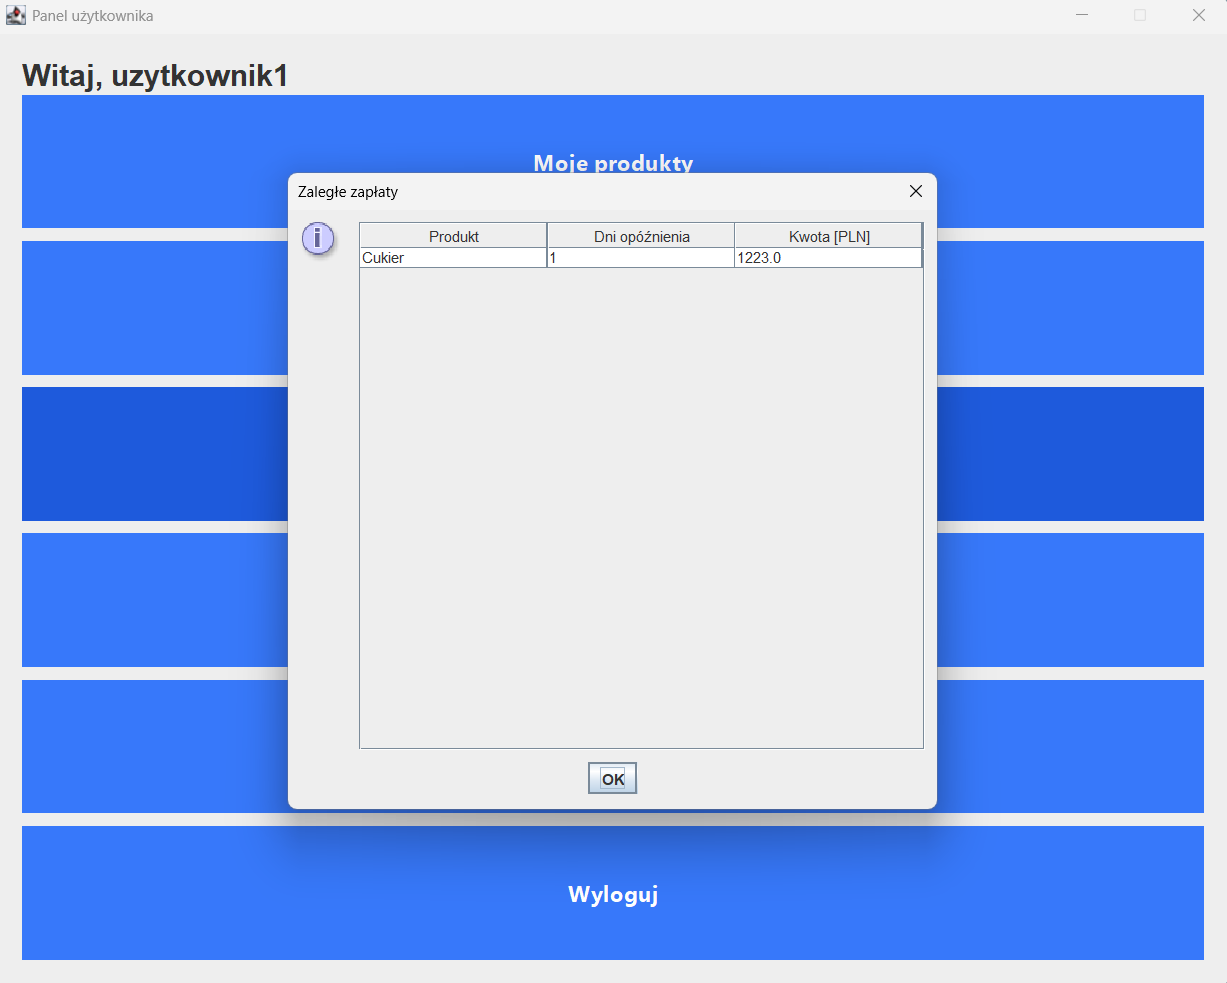
\includegraphics[width=.7\linewidth]{figures/PanelUzytkownika13.png}\
    \caption{PanelUzytkownika13.\label{PanelUzytkownika13}}
\end{figure}
\clearpage
\subsection{Cennik}
\label{subsec:Cennik}
Jeśli klikniemy na cennik to wyświetli nam się tabela:
\begin{figure}[H]
    \centering
    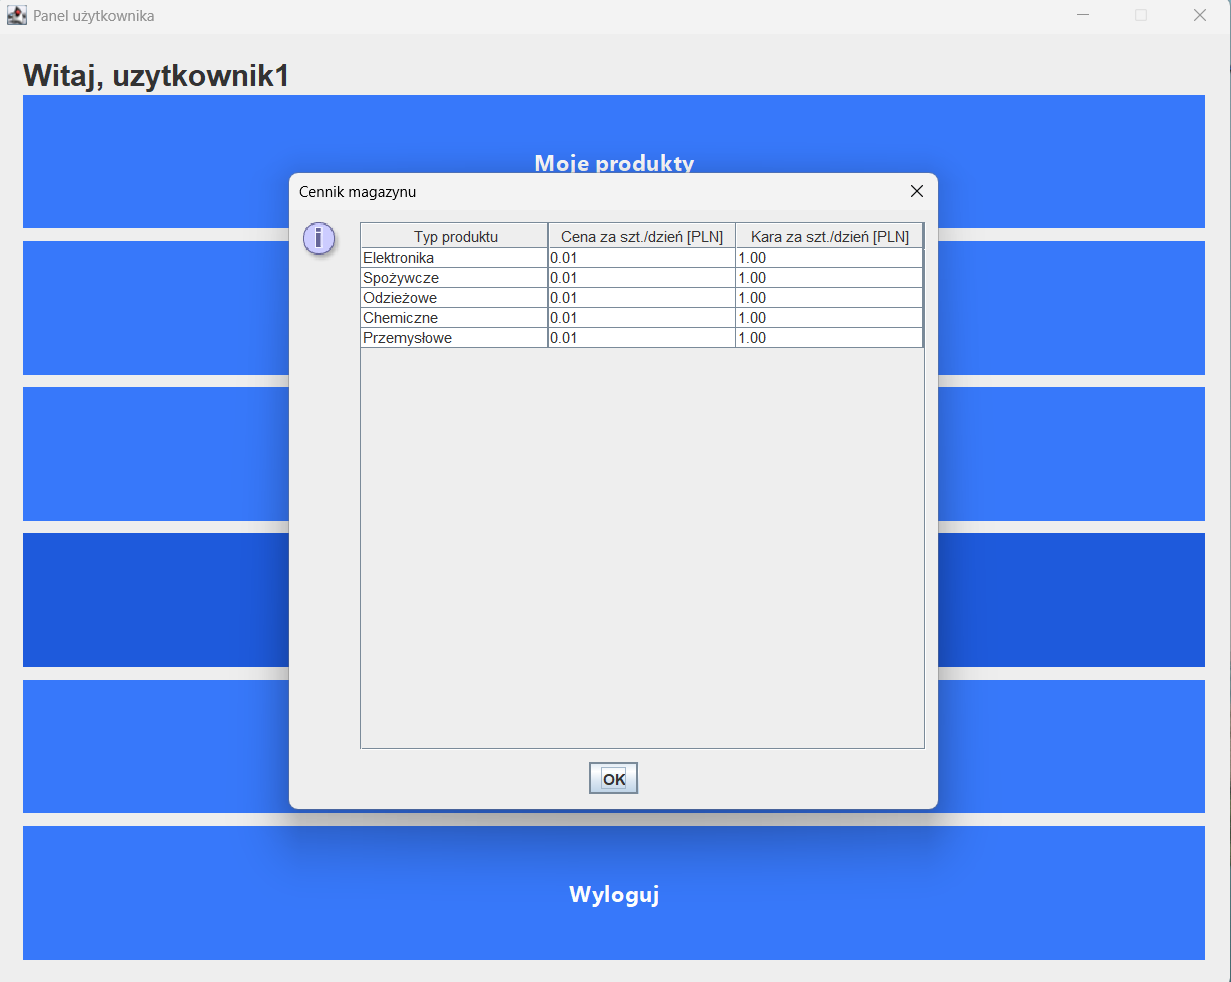
\includegraphics[width=.7\linewidth]{figures/PanelUzytkownika14.png}\
    \caption{PanelUzytkownika14.\label{PanelUzytkownika14}}
\end{figure}
\clearpage
\subsection{Zmień dane}
\label{subsec:Zmień dane}
Jeśli klikniemy na zmień dane to wyświetli się takie okno:
\begin{figure}[H]
    \centering
    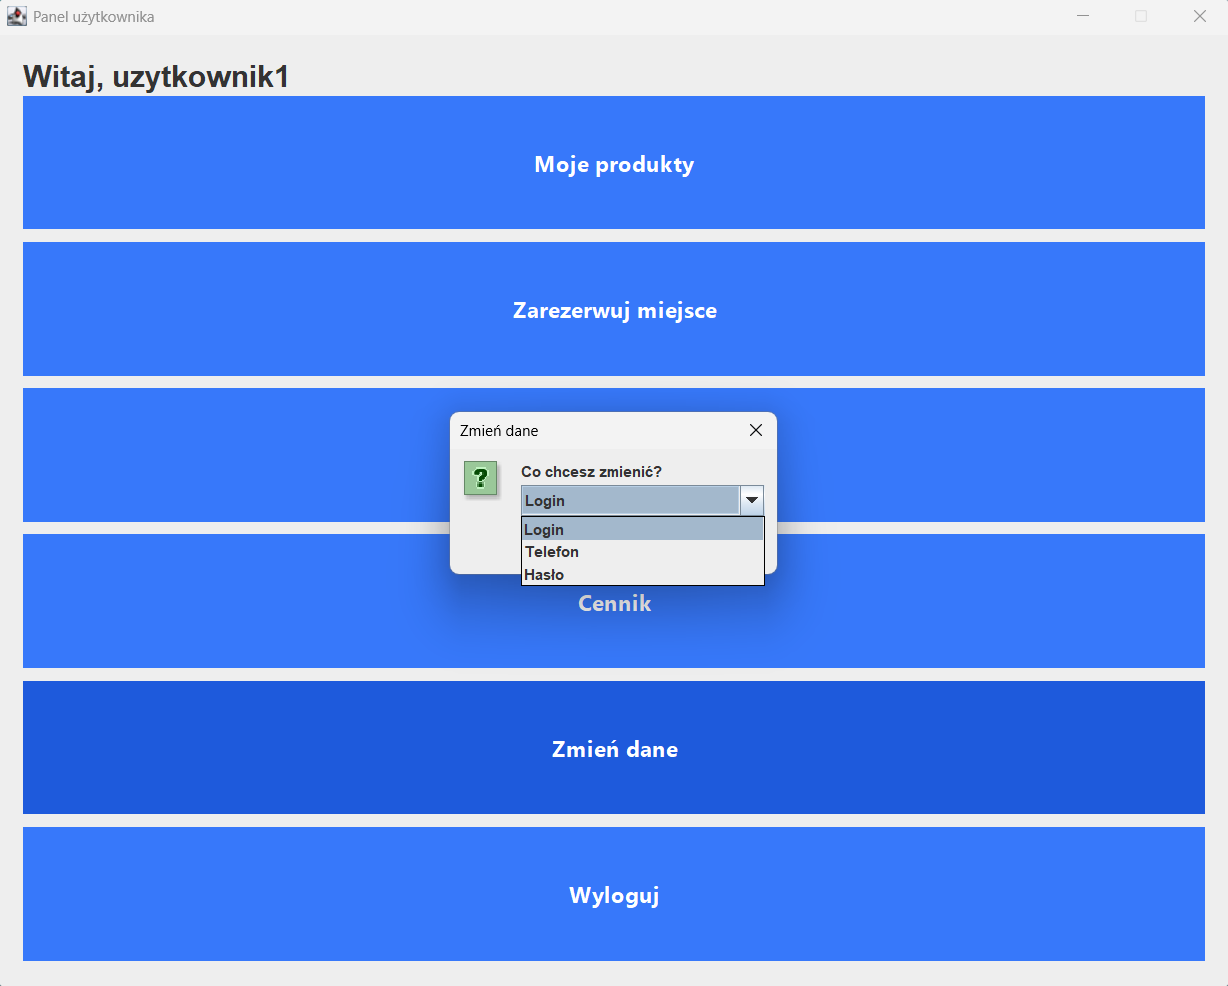
\includegraphics[width=.7\linewidth]{figures/PanelUzytkownika15.png}\
    \caption{PanelUzytkownika15.\label{PanelUzytkownika15}}
\end{figure}
Jeśli przy zmienianiu loginu nie będzie on miał 4 liter to wyświetli taki komunikat:
\begin{figure}[H]
    \centering
    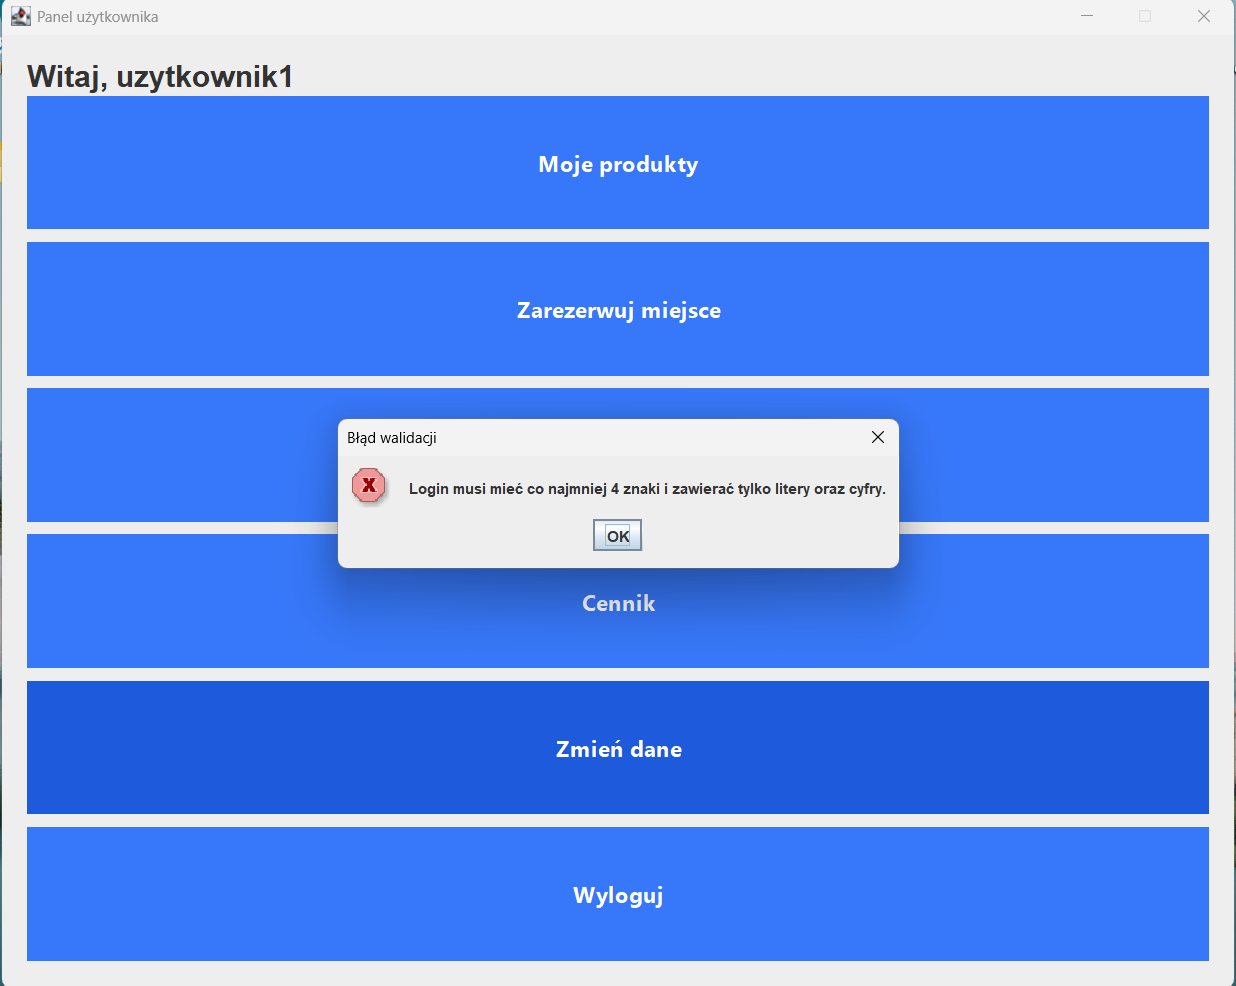
\includegraphics[width=.7\linewidth]{figures/PanelUzytkownika16.png}\
    \caption{PanelUzytkownika16.\label{PanelUzytkownika16}}
\end{figure}
Jeśli jednak login zostanie wpisany poprawnie to wyświetli się taki komunikat:
\begin{figure}[H]
    \centering
    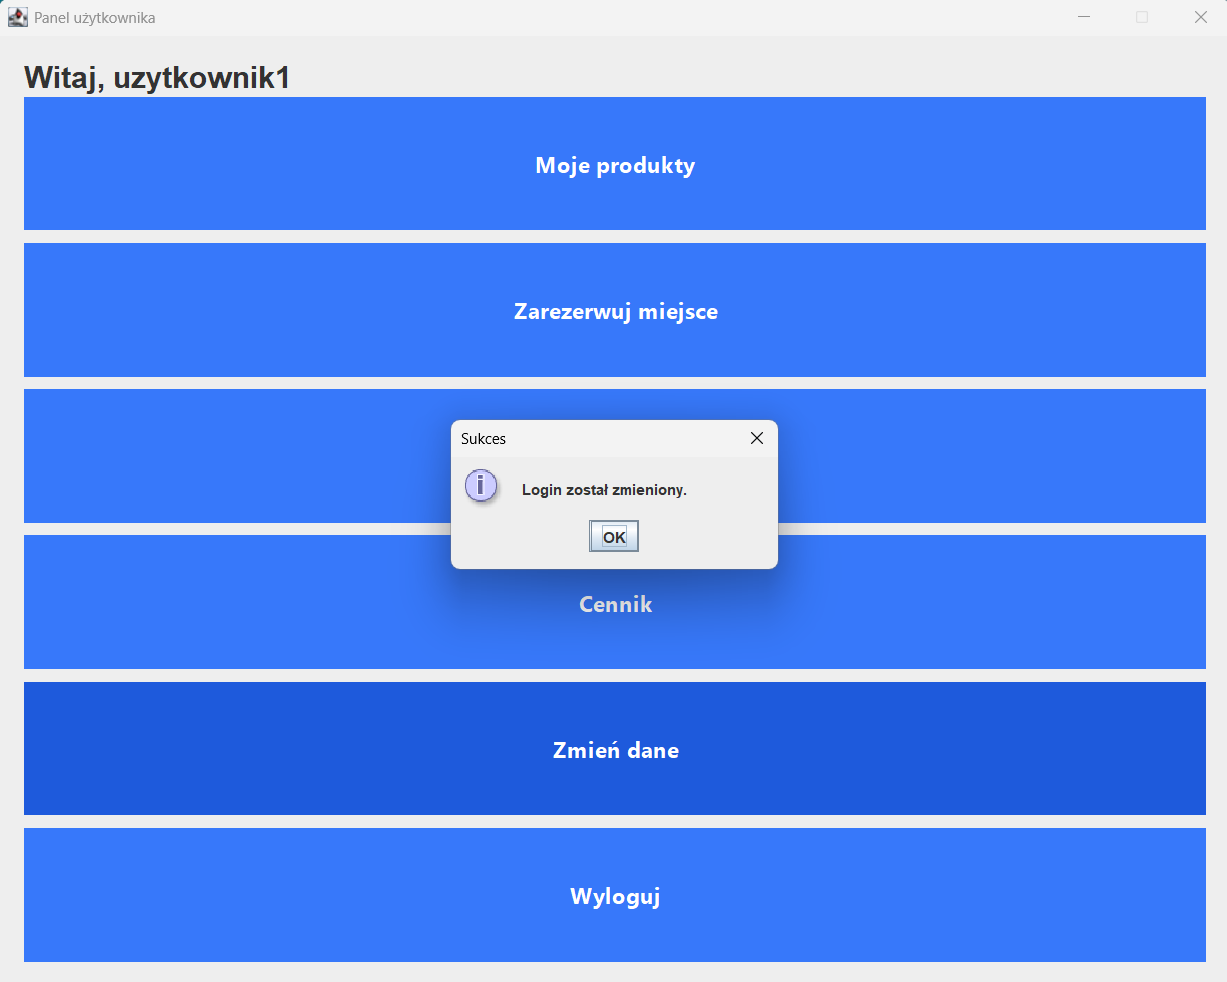
\includegraphics[width=.7\linewidth]{figures/PanelUzytkownika17.png}\
    \caption{PanelUzytkownika17.\label{PanelUzytkownika17}}
\end{figure}
Jeśli przy zmianie Nr.Tel nie będzie od 9 do 11 liter wyświetli taki komunikat:
\begin{figure}[H]
    \centering
    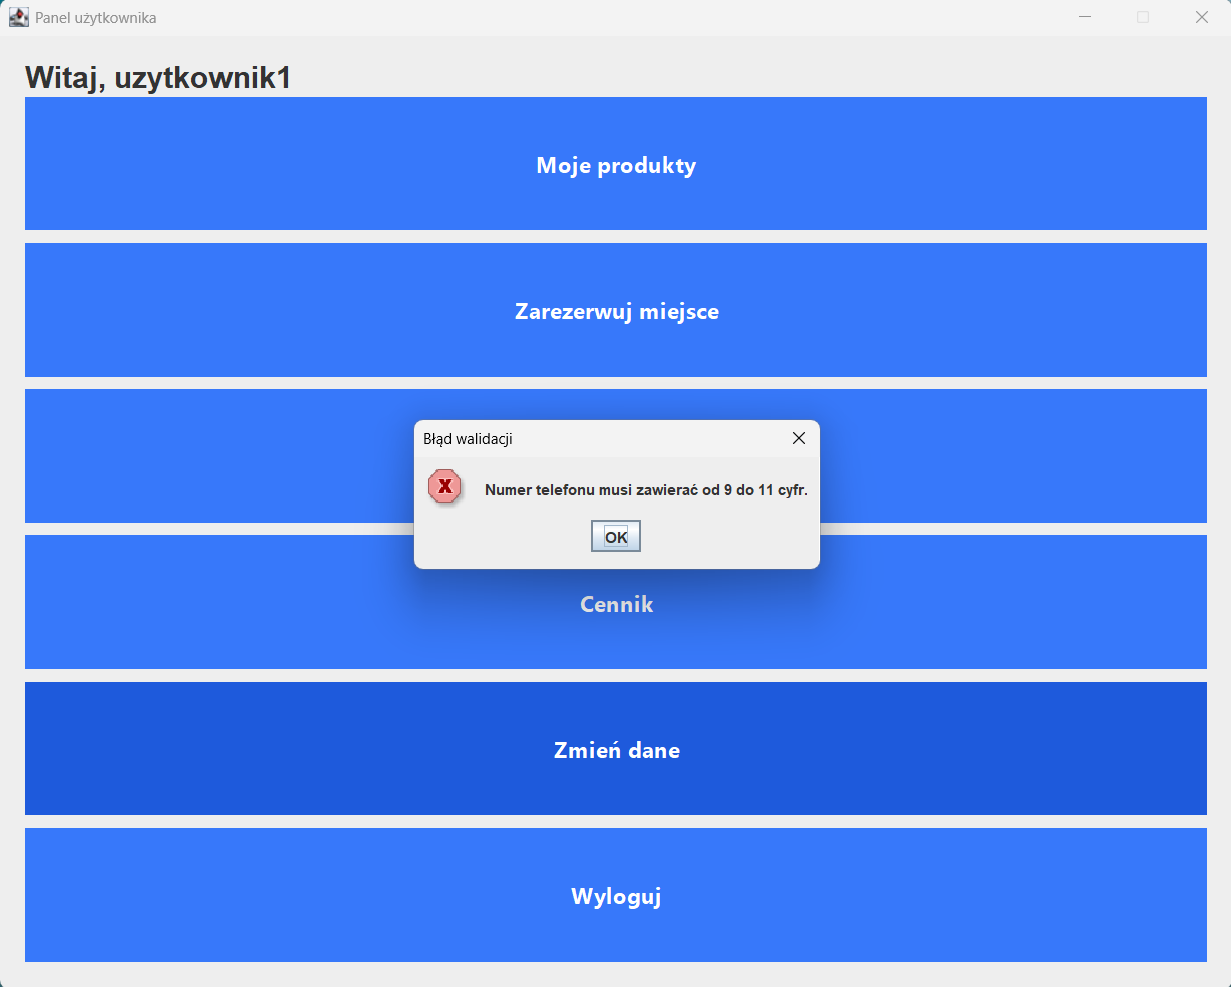
\includegraphics[width=.7\linewidth]{figures/PanelUzytkownika18.png}\
    \caption{PanelUzytkownika18.\label{PanelUzytkownika18}}
\end{figure}
Natomiast gdy użytkownik dobrze wpisze nowy Nr.Tel. wyświetli taki komunikat:
\begin{figure}[H]
    \centering
    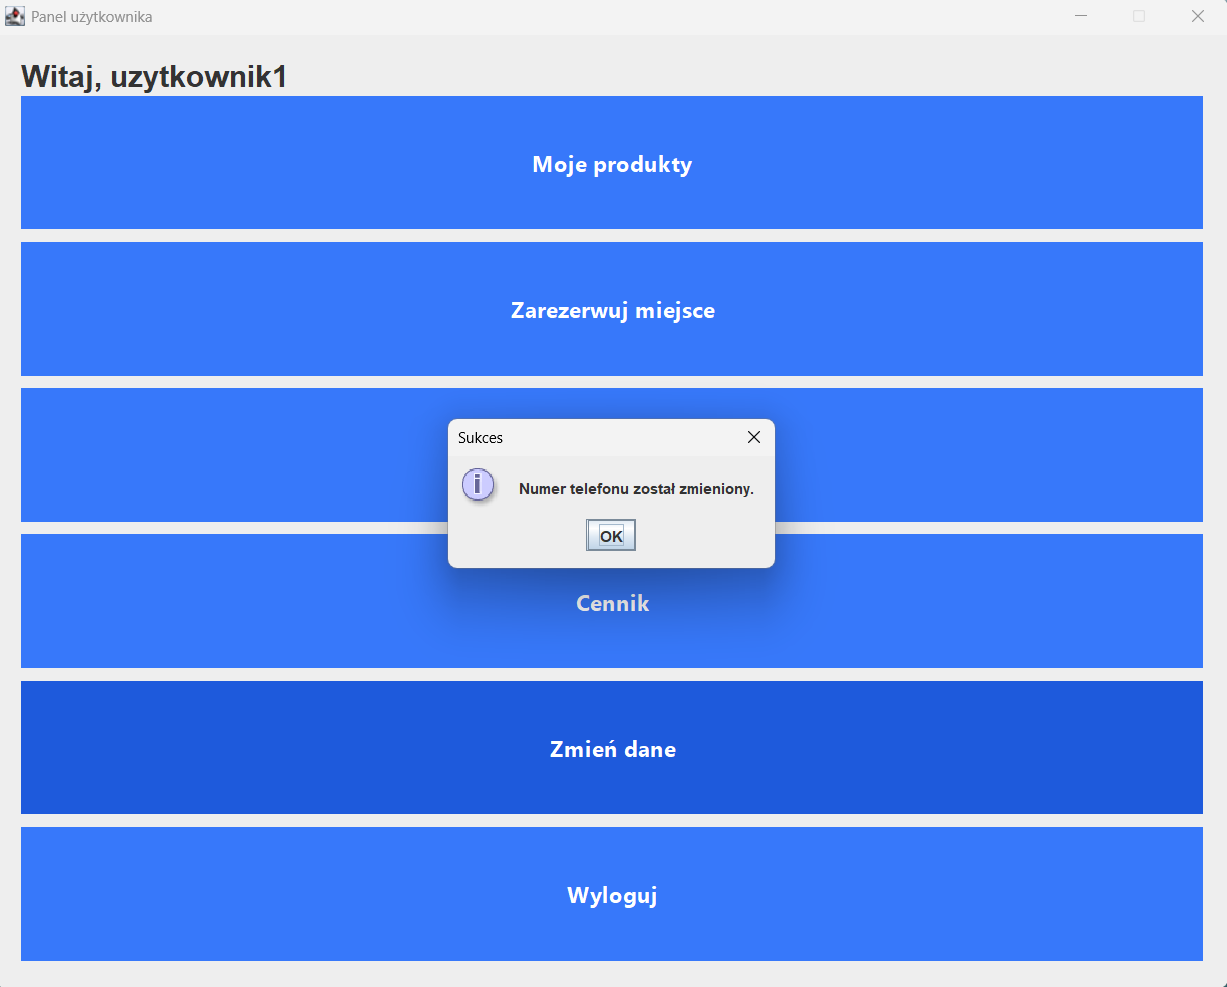
\includegraphics[width=.7\linewidth]{figures/PanelUzytkownika19.png}\
    \caption{PanelUzytkownika19.\label{PanelUzytkownika19}}
\end{figure}
Po wybraniu zmiany hasła, gdy nie będą się one pokrywać, wyświetli taki komunikat:
\begin{figure}[H]
    \centering
    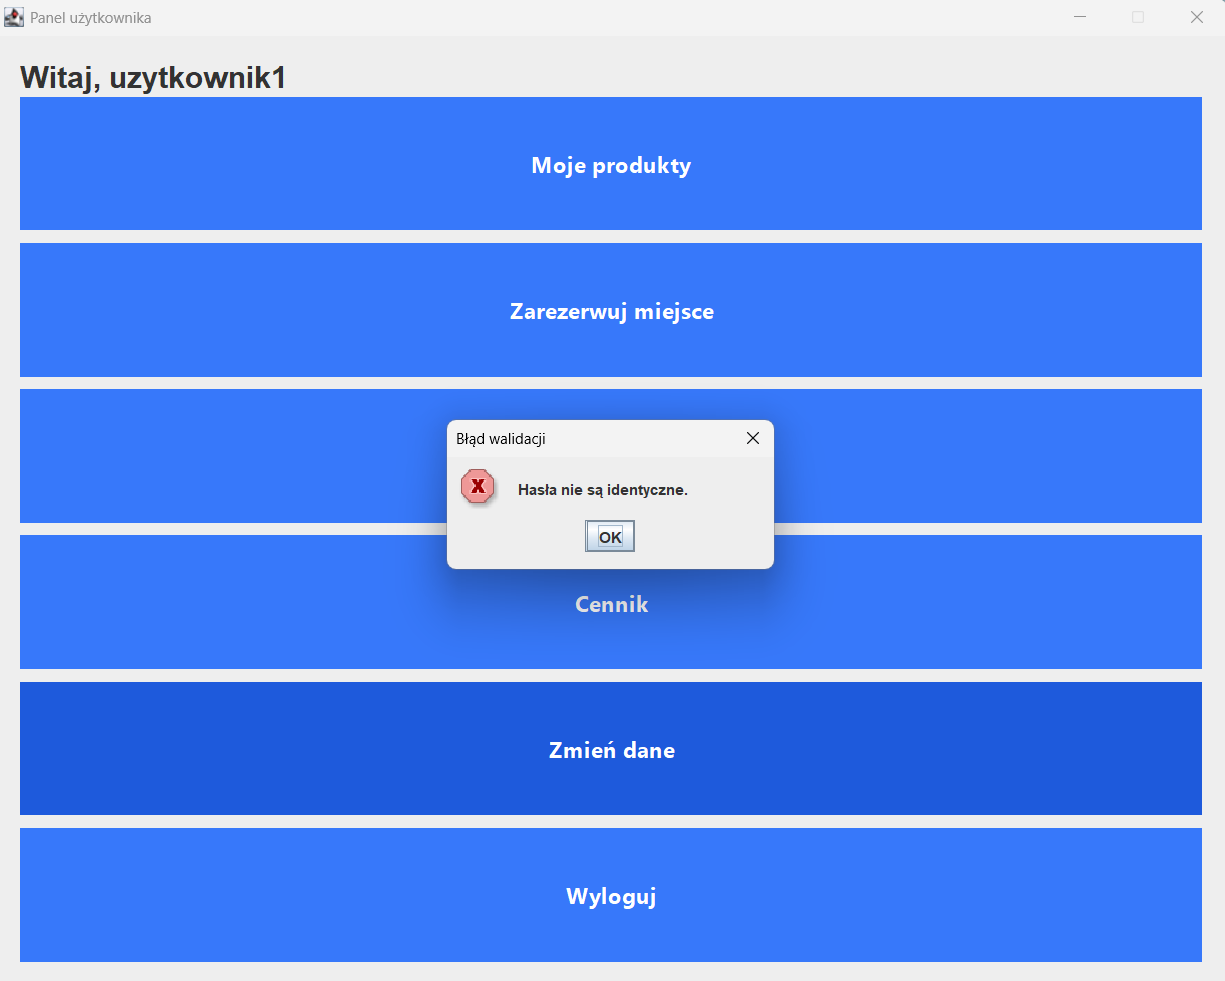
\includegraphics[width=.7\linewidth]{figures/PanelUzytkownika20.png}\
    \caption{PanelUzytkownika20.\label{PanelUzytkownika20}}
\end{figure}
Jeśli hasła się pokrywają:
\begin{figure}[H]
    \centering
    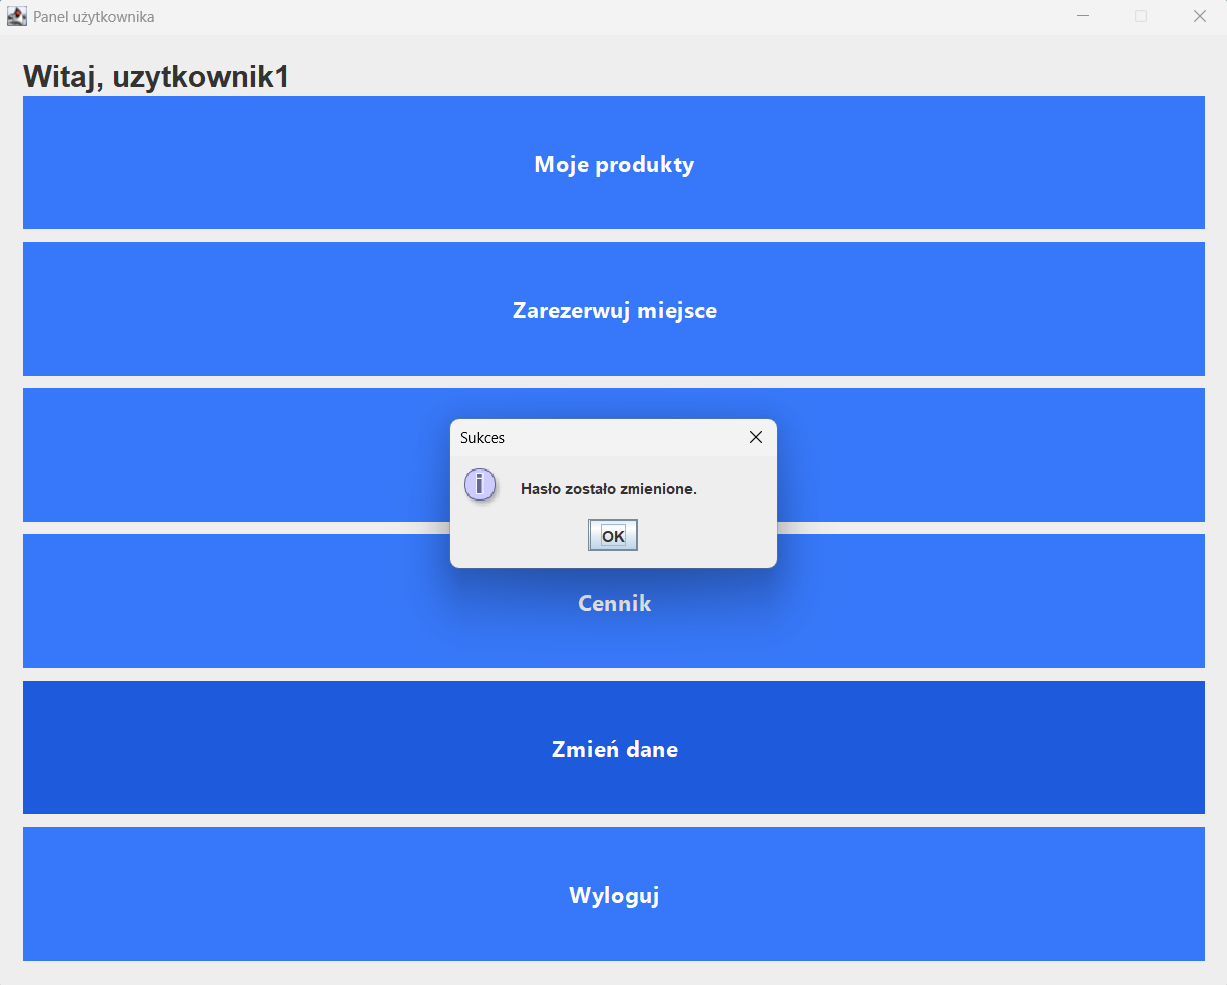
\includegraphics[width=.7\linewidth]{figures/PanelUzytkownika21.png}\
    \caption{PanelUzytkownika21.\label{PanelUzytkownika21}}
\end{figure}
\clearpage
\subsection{Wyloguj}
\label{subsec:Wyloguj}
Po kliknięciu przycisku Wyloguj wyświetli się komunikat:
\begin{figure}[H]
    \centering
    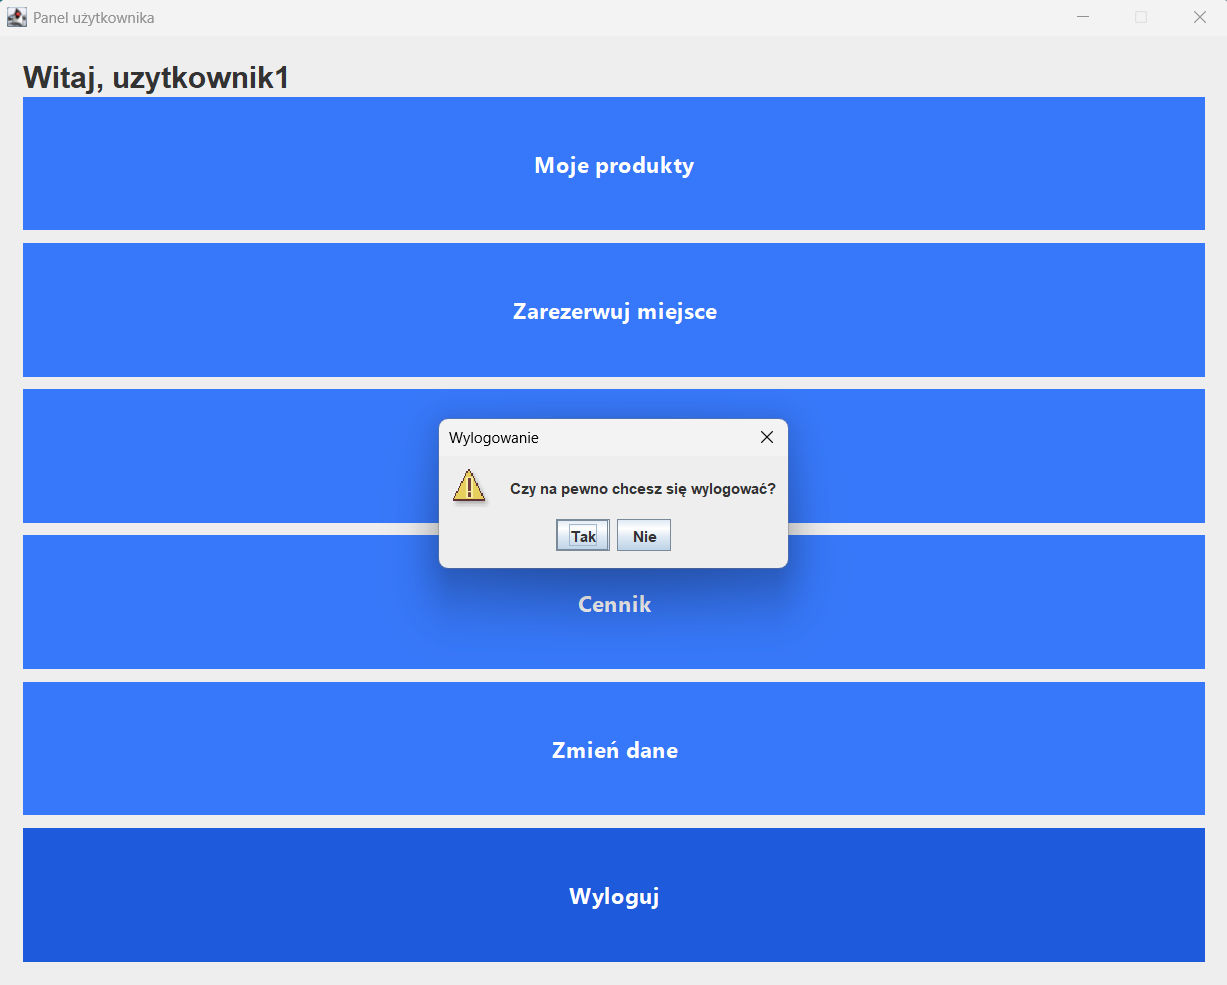
\includegraphics[width=.7\linewidth]{figures/PanelUzytkownika22.png}\
    \caption{PanelUzytkownika22.\label{PanelUzytkownika22}}
\end{figure}
\clearpage
\section{PanelAdministratora}
\label{sec:PanelAdministratora}
Jeśli w oknie logowania zalogujemy się na konto użytkownika będącego administratorem wyskoczy nam PanelAdministratora:
\begin{figure}[H]
    \centering
    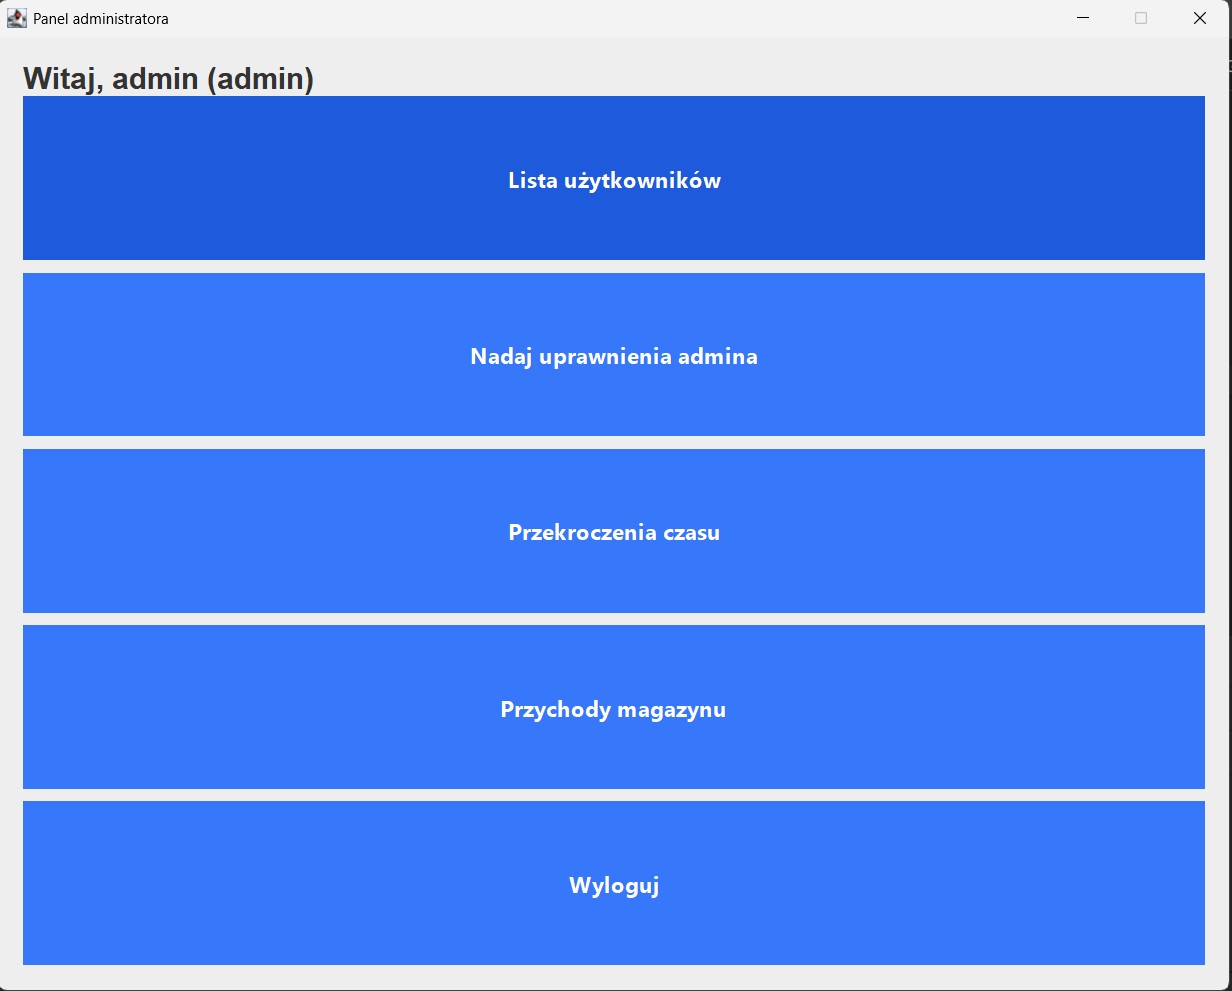
\includegraphics[width=.7\linewidth]{figures/PanelAdministratora.png}\
    \caption{PanelAdministratora.\label{PanelAdministratora}}
\end{figure}
\clearpage
\subsection{Lista użytkowników}
\label{subsec:Lista użytkowników}
Po kliknięciu na Lista użytkowników wyświetli się lista użytkowników wraz z ich produktami
\begin{figure}[H]
    \centering
    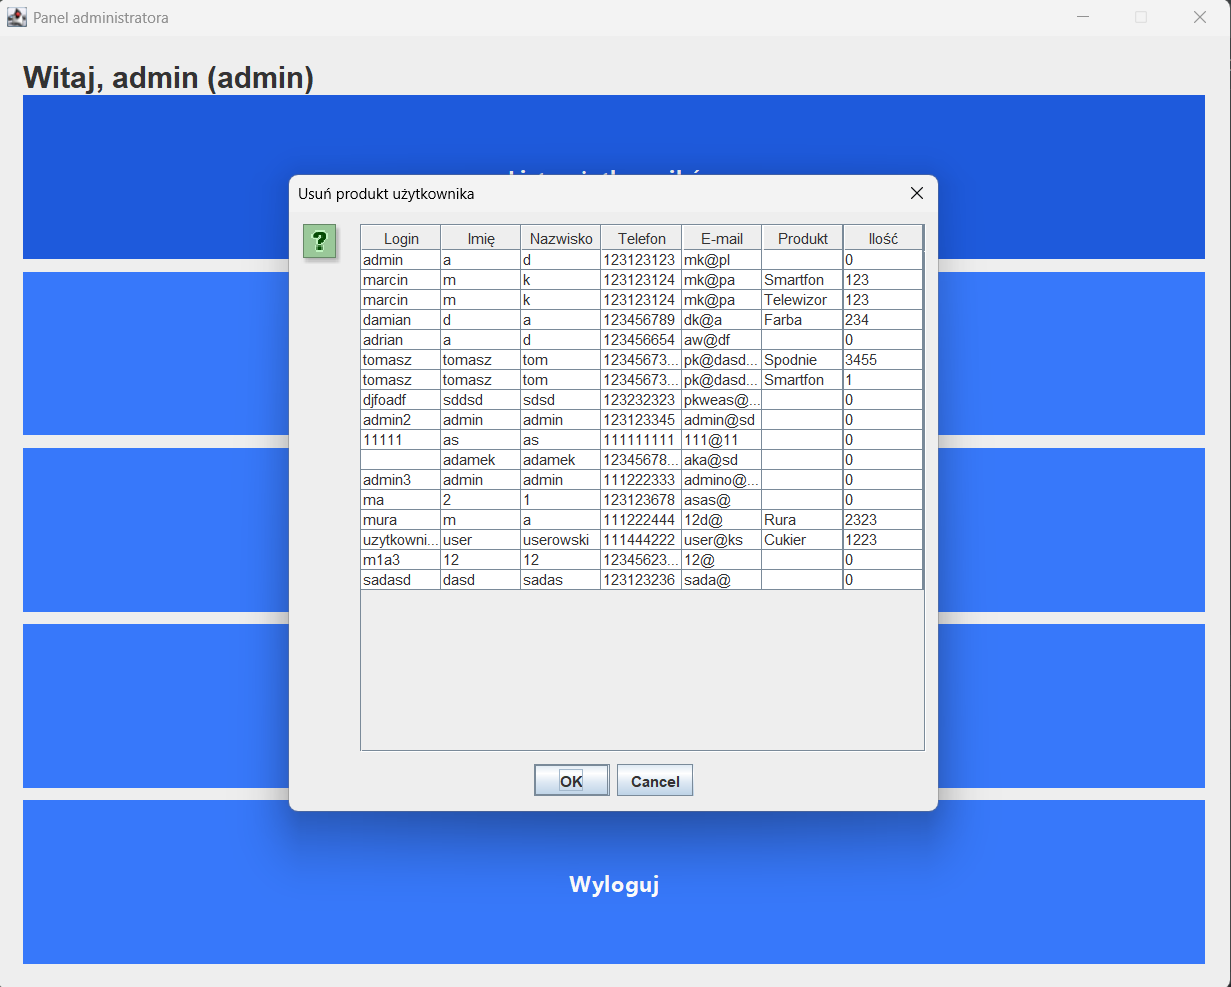
\includegraphics[width=.7\linewidth]{figures/PanelAdministratora1.png}\
    \caption{PanelAdministratora1.\label{PanelAdministratora1}}
\end{figure}
Jak zedytujemy coś w kolumnie ilość to usunie ten produkt z tego samego wiersza oraz wyda taki komunikat
\begin{figure}[H]
    \centering
    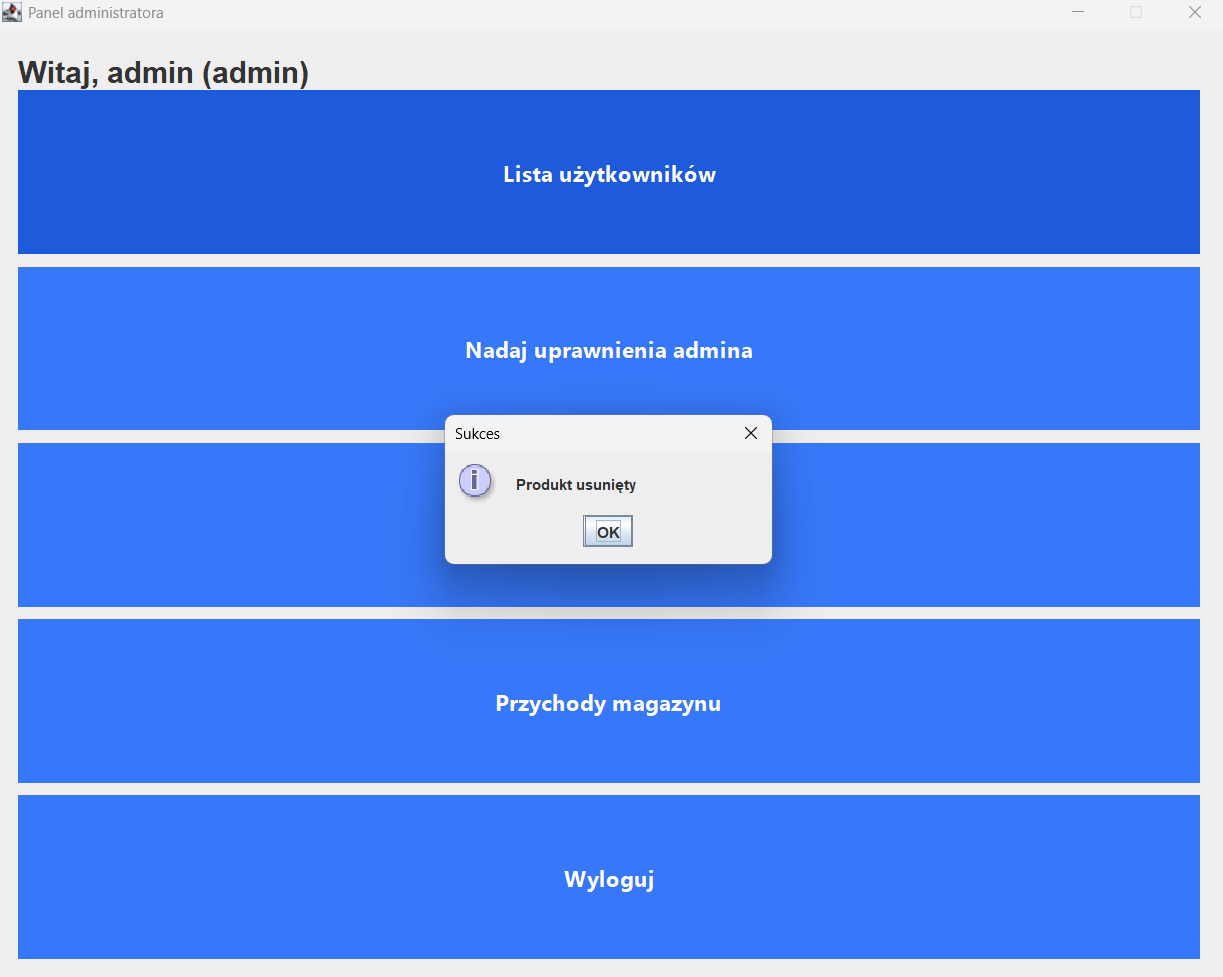
\includegraphics[width=.7\linewidth]{figures/PanelAdministratora2.png}\
    \caption{PanelAdministratora2.\label{PanelAdministratora2}}
\end{figure}
\clearpage
\subsection{Nadaj uprawnienia admina}
\label{subsec:Nadaj uprawnienia admina}
Po kliknięciu Nadaj uprawnienia admina wyświetla się takie okno 
\begin{figure}[H]
    \centering
    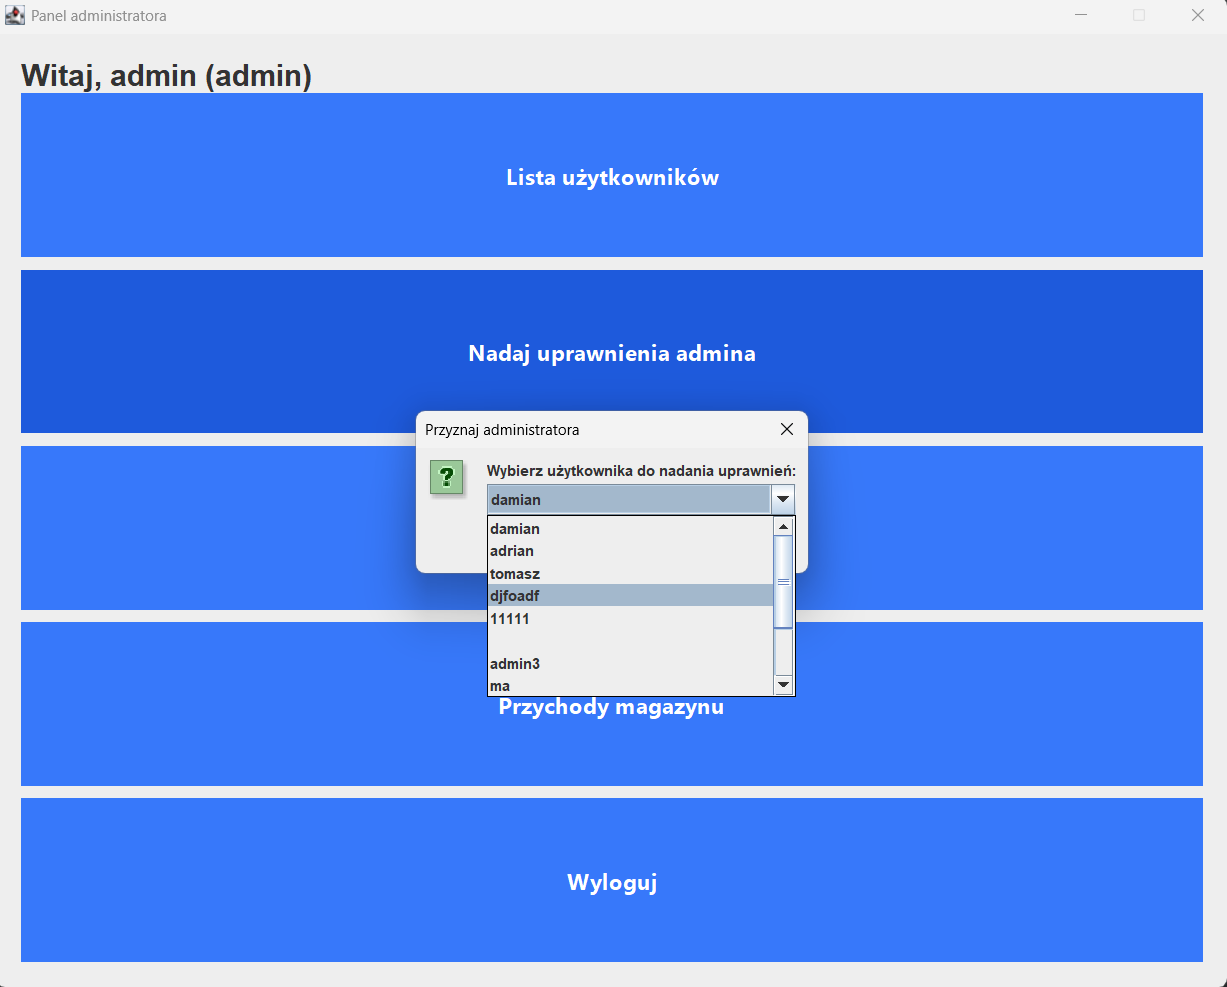
\includegraphics[width=.7\linewidth]{figures/PanelAdministratora3.png}\
    \caption{PanelAdministratora3.\label{PanelAdministratora3}}
\end{figure}
a po tym wyświetla komunikat:
\begin{figure}[H]
    \centering
    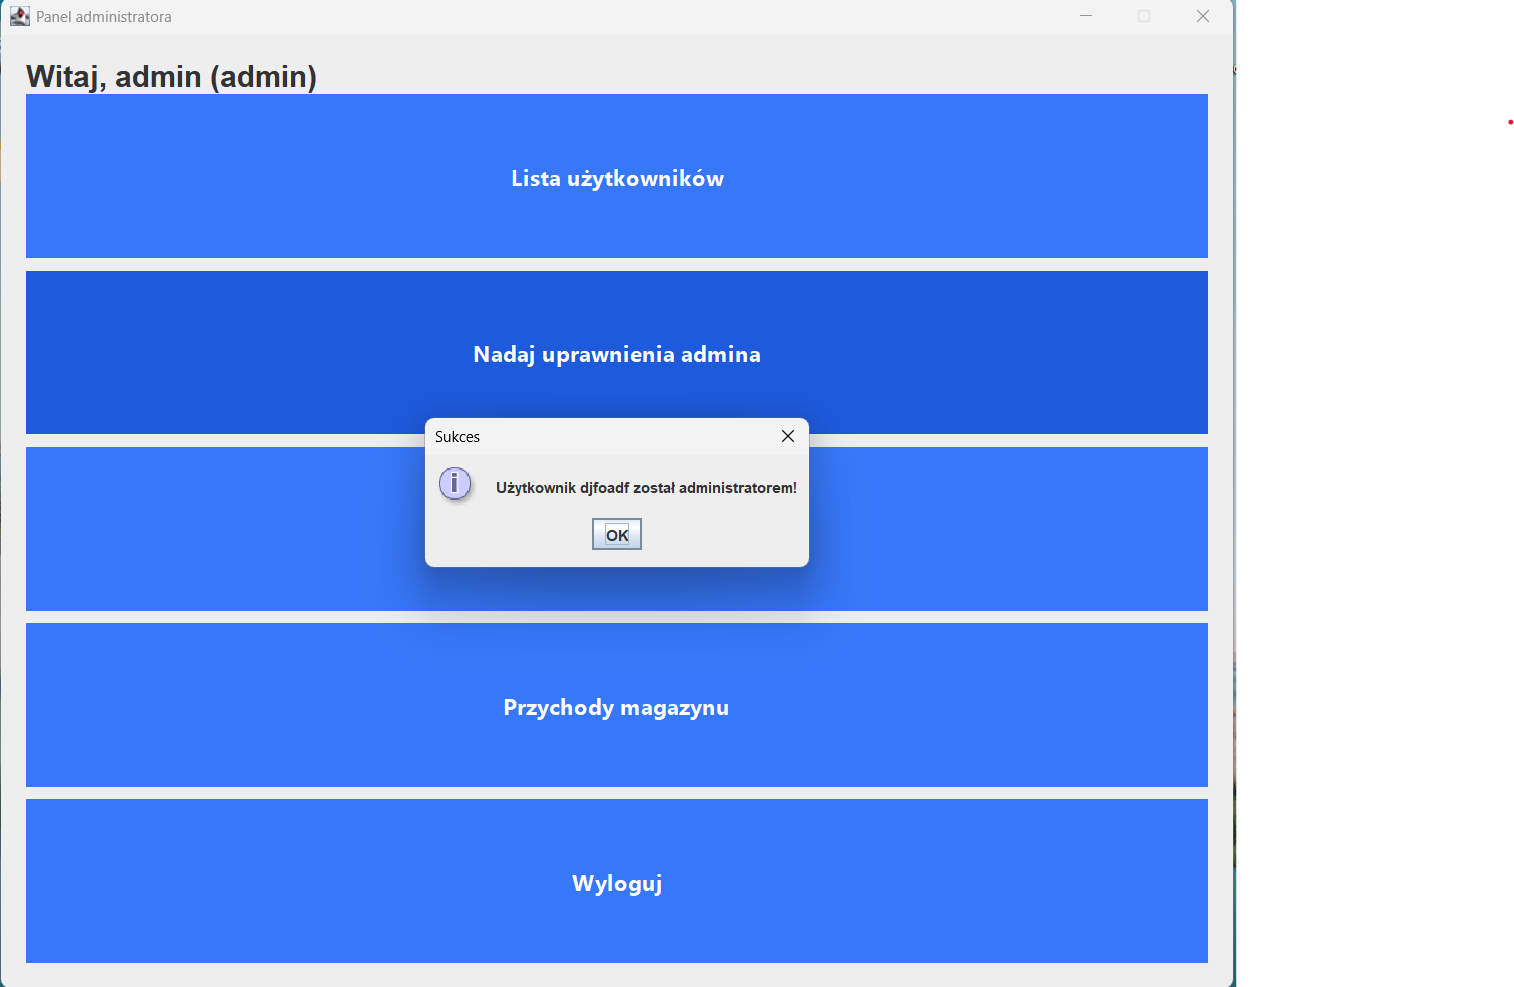
\includegraphics[width=.7\linewidth]{figures/PanelAdministratora5.png}\
    \caption{PanelAdministratora5.\label{PanelAdministratora5}}
\end{figure}
\clearpage
\subsection{Przekroczenia czasu}
\label{subsec:Przekroczenia czasu}
Gdy klikniemy Przekroczenia czasu wyświetli tabele z użytkownikami, którzy nie odebrali swojego materiału na czas
\begin{figure}[H]
    \centering
    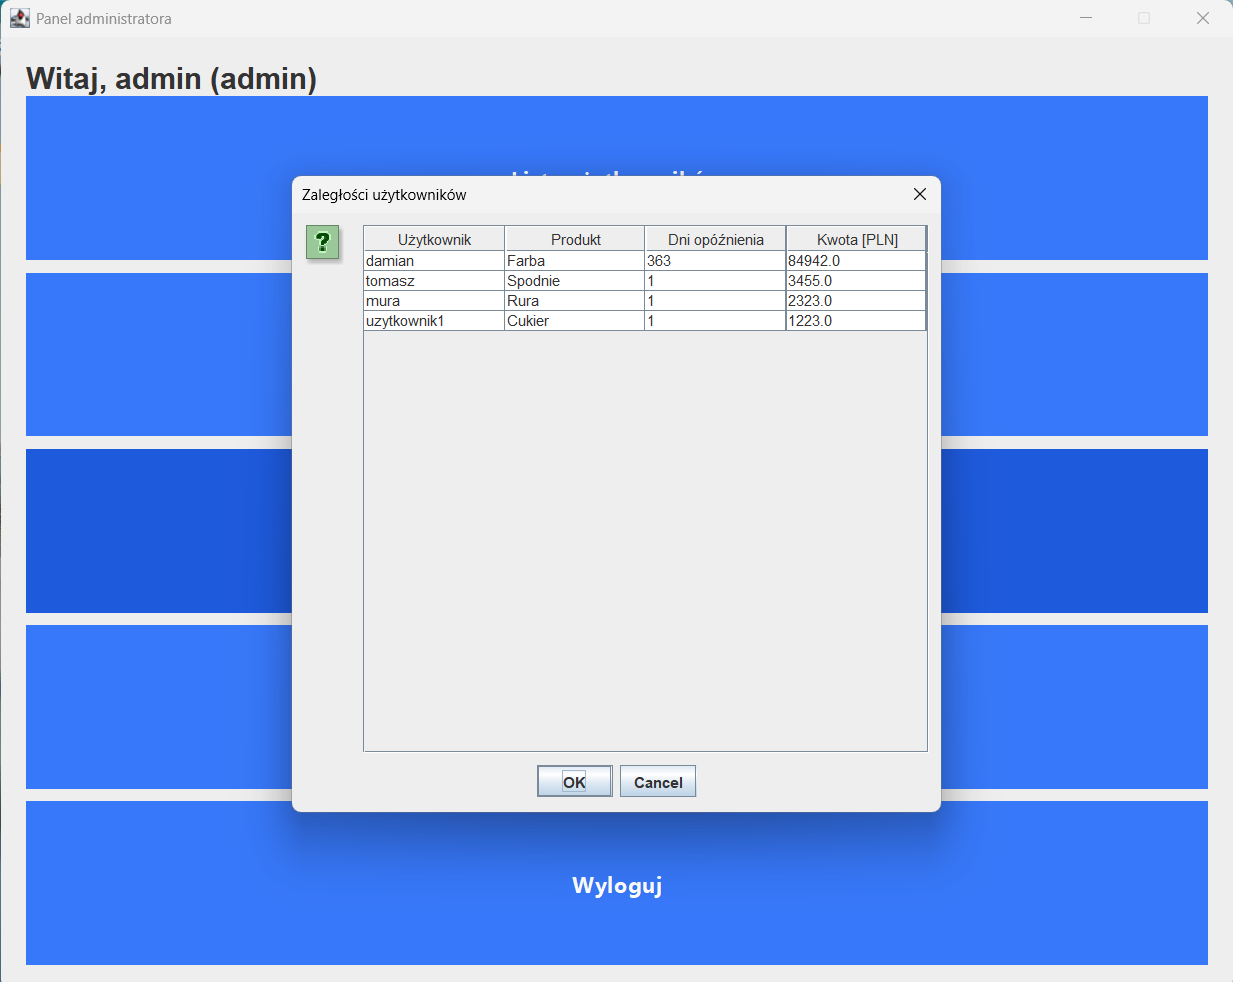
\includegraphics[width=.7\linewidth]{figures/PanelAdministratora6.png}\
    \caption{PanelAdministratora6.\label{PanelAdministratora6}}
\end{figure}
Jeśli zedytujemy coś w kolumnie kwota to usuwa uzytkownika z tego wiersza, w którym zedytowaliśmy kolumne kwota
\begin{figure}[H]
    \centering
    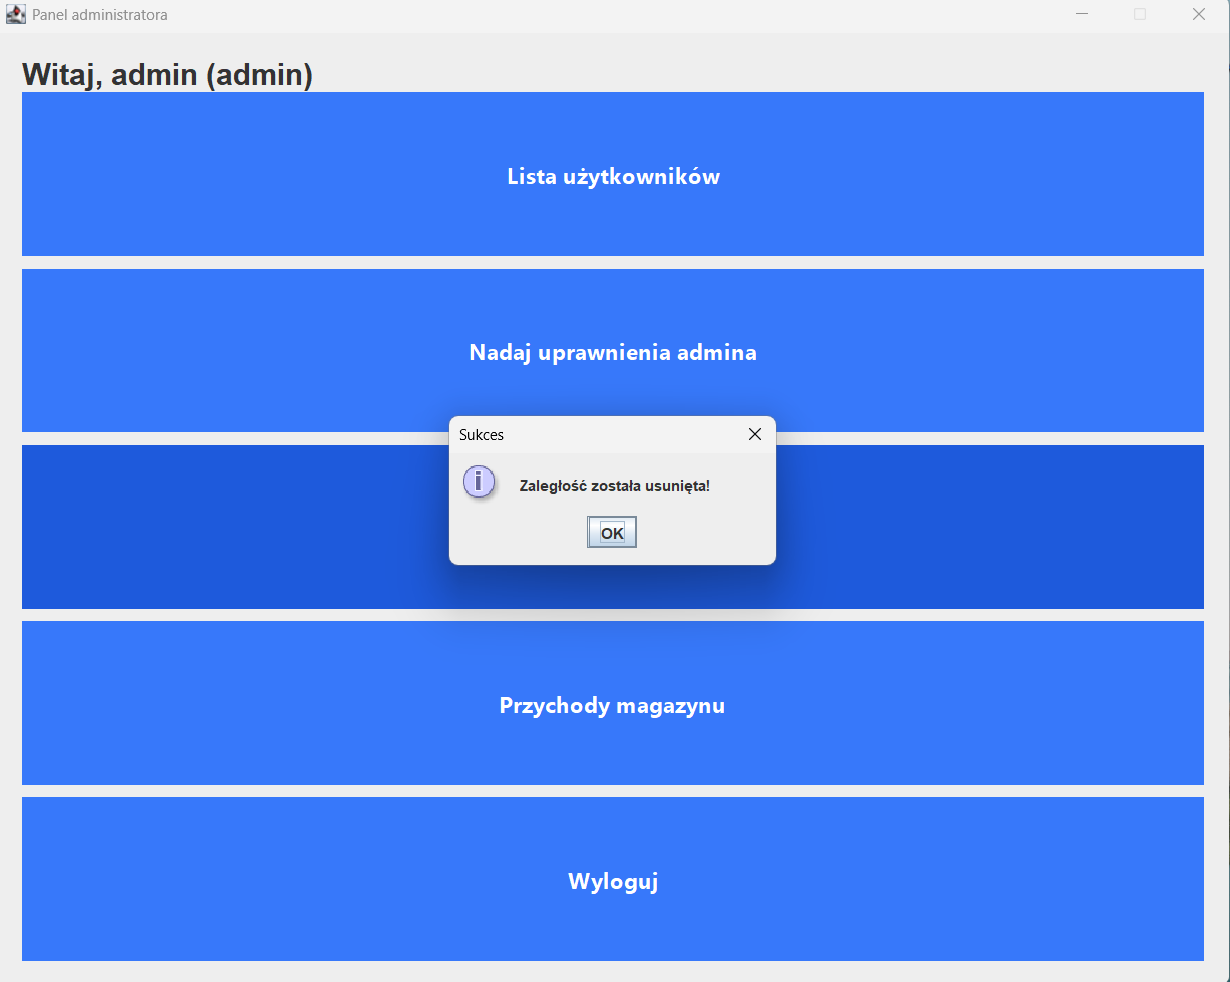
\includegraphics[width=.7\linewidth]{figures/PanelAdministratora7.png}\
    \caption{PanelAdministratora7.\label{PanelAdministratora7}}
\end{figure}
\clearpage
\subsection{Przychody magazynu}
\label{subsec:Przychody magazynu}
Wyświetla tabele z przychodami
\begin{figure}[H]
    \centering
    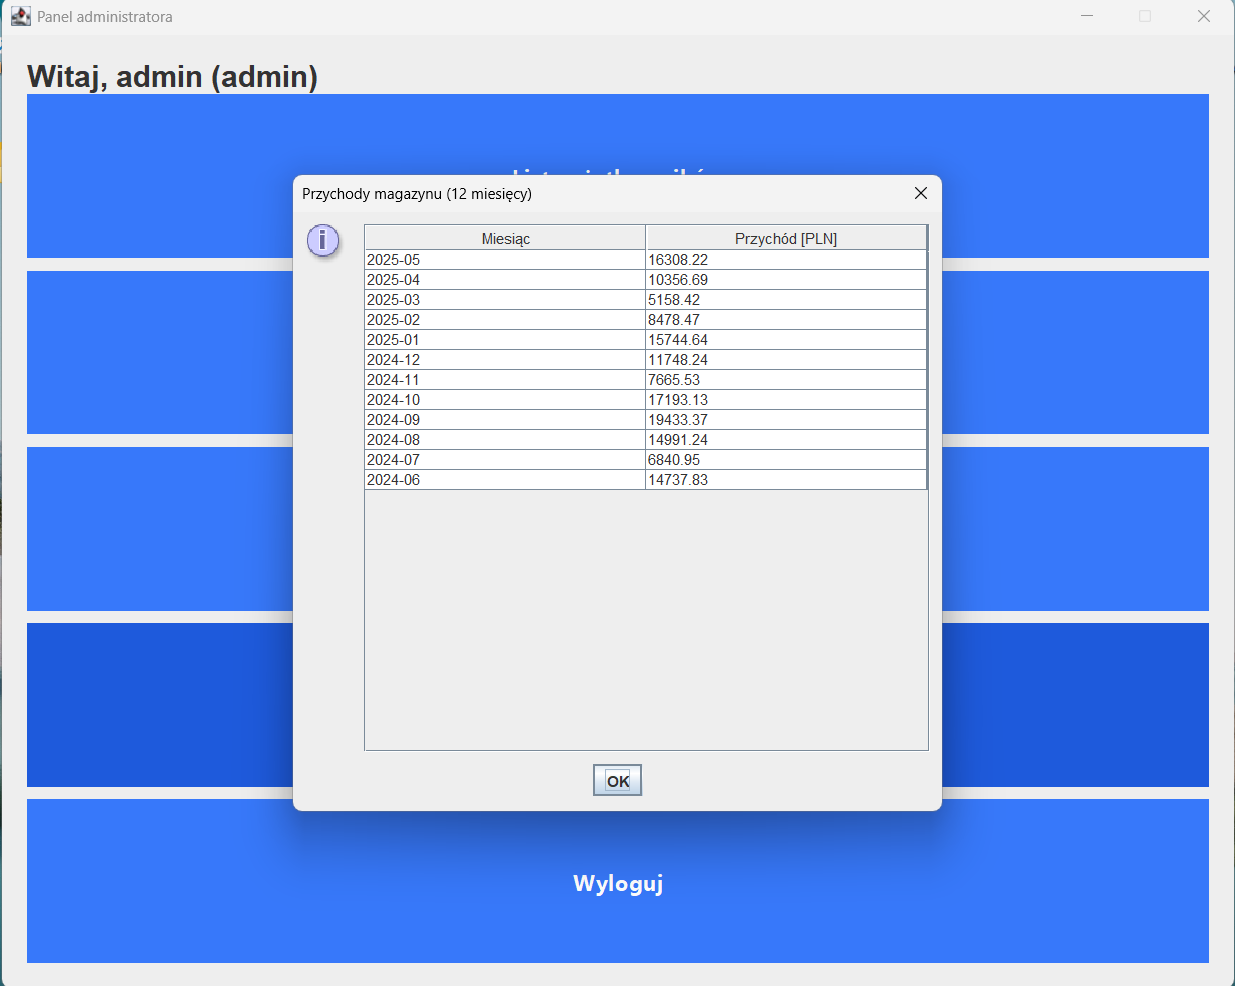
\includegraphics[width=.7\linewidth]{figures/PanelAdministratora8.png}\
    \caption{PanelAdministratora8.\label{PanelAdministratora8}}
\end{figure}
\clearpage
\subsection{Wyloguj}
\label{subsec:Wyloguj}
Po kliknięciu przycisku Wyloguj wyświetli się komunikat:
\begin{figure}[H]
    \centering
    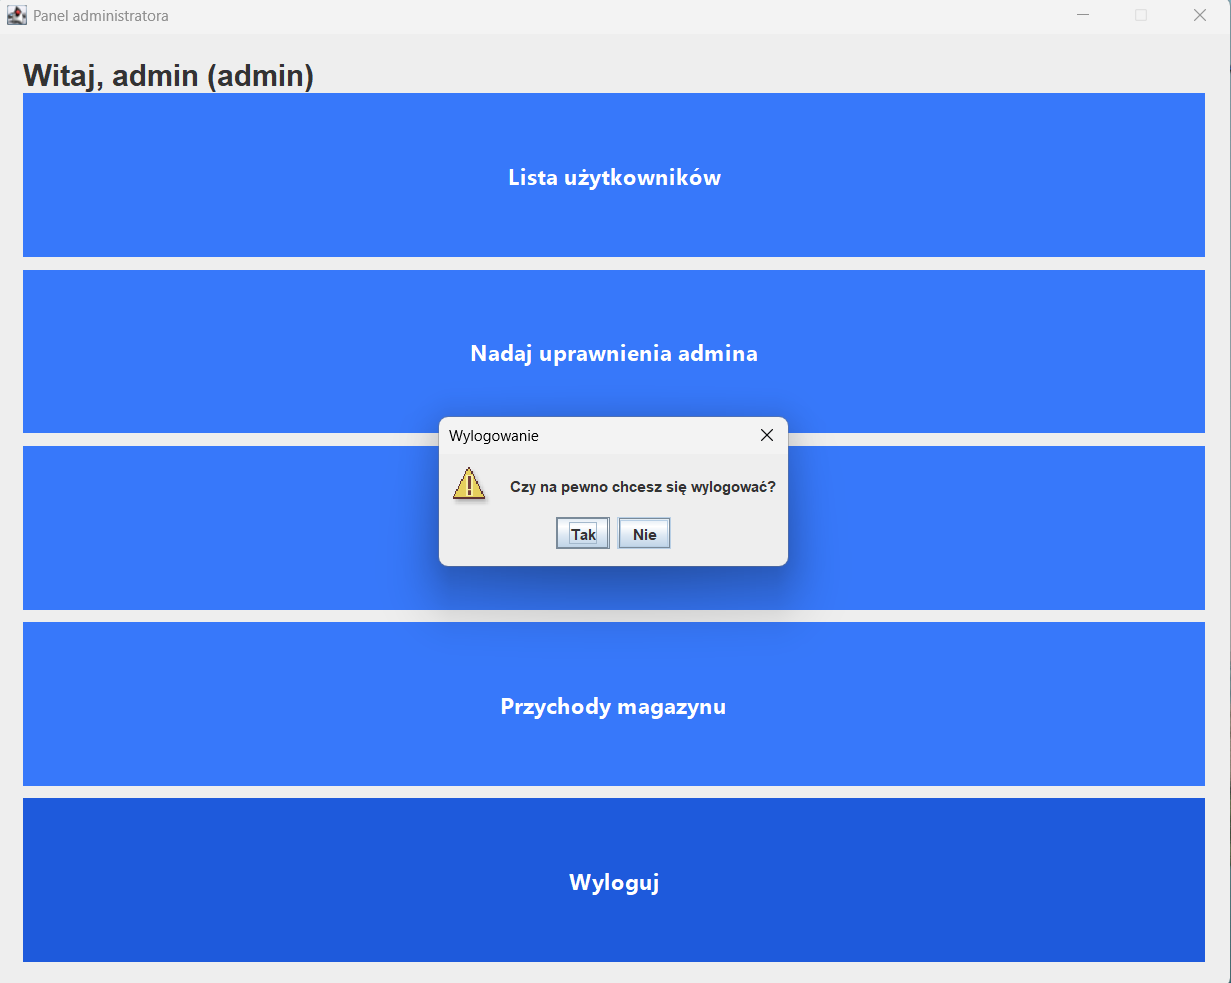
\includegraphics[width=.7\linewidth]{figures/PanelAdministratora9.png}\
    \caption{PanelAdministratora9.\label{PanelAdministratora9}}
\end{figure}
\chapter{Podsumowanie}
\label{chap:Podsumowanie}

\section{Zrealizowane elementy}
\label{sec:Zrealizowane elementy}
W projekcie zaimplementowano następujące funkcjonalności:

\subsection{System logowania i rejestracji}
\label{subsec:System logowania i rejestracji}
\begin{itemize}
\item Walidacja danych (login, hasło, e-mail, numer telefonu)
\item Podział na zwykłych użytkowników i administratorów
\end{itemize}

\subsection{Panel użytkownika}
\label{subsec:Panel użytkownika}
\begin{itemize}
\item Przegląd zarezerwowanych produktów
\item Rezerwacja miejsca w magazynie (wybór typu produktu, ilości, dat przyjęcia i odbioru)
\item Wyświetlanie zaległych płatności (kary za przekroczenie terminu)
\item Cennik usług magazynowych
\item Możliwość zmiany danych konta (login, hasło, numer telefonu)
\end{itemize}

\subsection{Panel administratora}
\label{subsec:Panel administratora}
\begin{itemize}
\item Zarządzanie użytkownikami (lista wszystkich kont)
\item Nadawanie uprawnień administratora
\item Przegląd zaległych zamówień (kary za opóźnienia)
\item Raporty przychodów magazynu (ostatnie 12 miesięcy)
\end{itemize}

\subsection{Baza danych}
\label{subsec:Baza danych}
\begin{itemize}
\item Przechowywanie danych użytkowników (\texttt{uzytkownicy})
\item Zarządzanie produktami (\texttt{produkty})
\item Śledzenie kar (\texttt{kary})
\item Rejestr przychodów (\texttt{transakcje})
\end{itemize}

\subsection{Interfejs graficzny (GUI)}
\label{subsec:Interfejs graficzny (GUI)}
\begin{itemize}
\item Spójny wygląd wszystkich okien (\texttt{OknoBazowe})
\item Responsywne przyciski (\texttt{WygladPrzyciskow})
\item Komunikaty błędów i potwierdzeń (\texttt{JOptionPane})
\end{itemize}

\section{Mozliwe prace rozwojowe}
\label{sec:Mozliwe prace rozwojowe}
Projekt można rozbudować o następujące funkcje:

\subsection{Bezpieczeństwo}
\label{subsec:Bezpieczeństwo}
\begin{itemize}
\item Hashowanie haseł (np. BCrypt) zamiast przechowywania ich w postaci jawnej
\item Weryfikacja dwuetapowa (np. SMS/e-mail)
\item Odzyskiwanie konta (zapomniałem hasła)
\end{itemize}

\subsection{Rozszerzenie funkcjonalności magazynu}
\label{subsec:Rozszerzenie funkcjonalności magazynu}
\begin{itemize}
\item Automatyczne naliczanie opłat (np. comiesięczne rozliczenia)
\item System powiadomień (e-mail/SMS o zbliżającym się terminie odbioru)
\item Generowanie faktur PDF po opłaceniu rezerwacji
\end{itemize}

\subsection{Dodatkowe moduły}
\label{subsec:Dodatkowe moduły}
\begin{itemize}
\item Panel dostawców – zarządzanie dostawami towarów
\item Historia transakcji – szczegółowe zestawienia płatności
\item Integracja z systemem płatności online (np. Przelewy24, PayPal)
\end{itemize}
\chapter{Podsumowanie}
\label{chap:Podsumowanie}

\section{Zrealizowane elementy}
\label{sec:Zrealizowane elementy}
W projekcie zaimplementowano następujące funkcjonalności:


SYSTEM LOGOWANIA I REJESTRACJI
\begin{itemize}
\item Walidacja danych (login, hasło, e-mail, numer telefonu)
\item Podział na zwykłych użytkowników i administratorów
\end{itemize}

PANEL UŻYTKOWNIKA
\begin{itemize}
\item Przegląd zarezerwowanych produktów
\item Rezerwacja miejsca w magazynie (wybór typu produktu, ilości, dat przyjęcia i odbioru)
\item Wyświetlanie zaległych płatności (kary za przekroczenie terminu)
\item Cennik usług magazynowych
\item Możliwość zmiany danych konta (login, hasło, numer telefonu)
\end{itemize}

PANEL ADMINISTRATORA
\begin{itemize}
\item Zarządzanie użytkownikami (lista wszystkich kont)
\item Nadawanie uprawnień administratora
\item Przegląd zaległych zamówień (kary za opóźnienia)
\item Raporty przychodów magazynu (ostatnie 12 miesięcy)
\end{itemize}

BAZA DANYCH
\begin{itemize}
\item Przechowywanie danych użytkowników (\texttt{uzytkownicy})
\item Zarządzanie produktami (\texttt{produkty})
\item Śledzenie kar (\texttt{kary})
\item Rejestr przychodów (\texttt{transakcje})
\end{itemize}

INTERFEJS GRAFICZNY
\begin{itemize}
\item Spójny wygląd wszystkich okien (\texttt{OknoBazowe})
\item Responsywne przyciski (\texttt{WygladPrzyciskow})
\item Komunikaty błędów i potwierdzeń (\texttt{JOptionPane})
\end{itemize}

\section{Mozliwe prace rozwojowe}
\label{sec:Mozliwe prace rozwojowe}
Projekt można rozbudować o następujące funkcje:

\begin{itemize}
\item Hashowanie haseł zamiast przechowywania ich w postaci jawnej
\item Weryfikacja dwuetapowa (np. SMS/e-mail)
\item Odzyskiwanie konta (zapomniałem hasła)
\item Automatyczne naliczanie opłat (np. comiesięczne rozliczenia)
\item System powiadomień (e-mail/SMS o zbliżającym się terminie odbioru)
\item Generowanie faktur PDF po opłaceniu rezerwacji
\item Historia transakcji - szczegółowe zestawienia płatności
\item Integracja z systemem płatności online (np. Przelewy24, PayPal)
\end{itemize}



% Wyłączenie działania `ulem` na czas bibliografii
\renewcommand{\emph}[1]{\textit{#1}}
% Bibliografia
% Dodanie bibliografi do spisu treści
\addcontentsline{toc}{section}{\textbf{Bibliografia}}
\bibliographystyle{plain}
\bibliography{bibliografia}

% Przywrócenie działania `ulem`
\renewcommand{\emph}[1]{\uline{#1}}

\clearpage
% Dodanie spisu rysunków do spisu treści
\addcontentsline{toc}{section}{\textbf{Spis rysunków}}
\listoffigures
\clearpage

% Dodanie spisu tabel do spisu treści
\addcontentsline{toc}{section}{\textbf{Spis tabel}}
\listoftables
\clearpage


\clearpage

% Dodanie spisu listingow do spisu treści
\addcontentsline{toc}{section}{\textbf{Spis listingów}}
\lstlistoflistings
\clearpage


% \appendix
\chapter*{}
\label{cha:statement-A}
\makeatletter
\addcontentsline{toc}{section}{\textbf{Oświadczenie studenta o samodzielności pracy}}

\noindent
\begin{flushright}
    \begin{minipage}[!h]{10cm}
        Załącznik nr 2 do Zarządzenia nr 228/2021 Rektora Uniwersytetu Rzeszowskiego z dnia 1 grudnia 2021 roku w sprawie ustalenia procedury antyplagiatowej w Uniwersytecie Rzeszowskim
    \end{minipage}
\end{flushright}

\begin{center}
    \vspace*{10mm}
    \noindent  {\textbf{OŚWIADCZENIE STUDENTA O SAMODZIELNOŚCI PRACY} }
    \vspace*{10mm}
\end{center}

\noindent
\dotuline{\hspace{1.3cm}\@author\hspace{1.3cm}}\\ % Linia pozioma
{\small Imię (imiona) i nazwisko studenta }\\

\noindent \@faculty\\

\noindent \dotuline{\hspace{1.4cm}\@degreeprogramme \hspace{1.4cm}}\\
{\small Nazwa kierunku} \\

\noindent \dotuline{\hspace{1.8cm}\@noAlbum\hspace{1.9cm}}\\
{\small Numer albumu}

\begin{enumerate}
    \item Oświadczam, że moja praca projektowa pt.: \@titlePL
          \begin{enumerate}[label=\arabic*)]
              \item została przygotowana przeze mnie samodzielnie*,
              \item nie narusza praw autorskich w rozumieniu ustawy z dnia 4 lutego 1994 roku o prawie autorskim i prawach pokrewnych (t.j. Dz.U. z 2021 r., poz. 1062) oraz dóbr osobistych chronionych prawem cywilnym,
              \item nie zawiera danych i informacji, które uzyskałem/am w sposób niedozwolony,
              \item nie była podstawą otrzymania oceny z innego przedmiotu na uczelni wyższej ani mnie, ani innej osobie.
          \end{enumerate}
    \item Jednocześnie wyrażam zgodę/nie wyrażam zgody** na udostępnienie mojej pracy projektowej do celów naukowo--badawczych z poszanowaniem przepisów ustawy o prawie autorskim i prawach pokrewnych.
\end{enumerate}


\vspace*{10mm}

\noindent
\underline{\hspace{6cm}} \hfill \underline{\hspace{6cm}} \\ % Puste miejsce na miejscowość, data oraz podpis
\hspace*{13mm}(miejscowość, data)  \hspace*{63mm}(czytelny podpis studenta)
\vspace*{10mm}

\vfill
\noindent
* Uwzględniając merytoryczny wkład prowadzącego przedmiot \\
** -- niepotrzebne skreślić


\end{document}
